\chapter{ARCHITECTURAL DESIGN}
\label{ch:architecturalDesign}%
% The \label{...}% enables to remove the small indentation that is generated, always leave the % symbol.

\section{Overview}
\label{sec:overview}
\paragraph{eMSP}
The eMSP Application is going to be a distributed one and it will be divided into three software levels (tiers): presentation, logic and data. This tier division is used in order to have maintainability and scalability.
\begin{enumerate}
    \item \textbf{Presentation: }All the components that will be used in order to provide the final user interfaces. They are provided by the Mobile Application. 
    \item \textbf{Logic: }All the components that contain logic for processing data. Since the Mobile Application is going to be a fat client (both presentation and logic) some of the logic components will be contained in it, meanwhile, the other components will be located on the Application Server.
    \item \textbf{Data: }All the components which implement storage and management of data. This includes DBMS and databases.
\end{enumerate}
The interaction between different entities will be handled by the logic tier which will include specific components able to grant these types of interactions:
\begin{itemize}
    \item Mobile Application - eMSP Application Server
    \item Mobile Application - external APIs
    \item eMSP Application Server - CPMSs
    \item eMSP Application Server - external APIs
\end{itemize}
\paragraph{CPMS}
The CPMS application will be instead a monolithic application that will include all the aforementioned tiers in just one single application. A monolithic application is better than a three-tier architecture for the CPMS application due to
\begin{itemize}
    \item \textbf{Simplicity}: Developers can easily understand the overall structure and apport small changes if requested by the CPO
    \item \textbf{Deployment}: The application is easy to deploy and can be contained in a single package ready to be executed by a server owned by the CPO
    \item \textbf{Integration}: Since the application's interfaces are well-defined and consistent it will be easier to integrate with other applications such as the eMSP.
\end{itemize}
During the development of the subsystem, it is important to consider how the eMSP and the CPMSs will communicate. When the eMSP needs to perform an operation on a specific CPMS (such as starting the charging process), it will send a request with the specific operation. Additionally, whenever there is a relevant update to charging station data, the CPMS will send the updated data to all previously associated eMSPs through a specific component. This asynchronous method of reading data for the charging stations is necessary because it allows the eMSP to store all updated data from the CPMS, improving scalability for drivers. If the data were read synchronously, the eMSP would need to send a request to the specific CPMS every time a driver wants to check charging station information, which could reduce scalability as the number of drivers increases.
\section{Component View} %AS
\label{sec:componentView}
In this section, the component view of the two systems is presented with a high level component diagram, which also highlights external interface interaction. \\% highlevel diagram
In the following sections, detailed diagrams are constructed in the same manner as described in section \ref{sec:overview}, with three tiers for the eMSP and a monolithic approach for the CPMS.
\newgeometry{left=1cm, bottom=1cm, includefoot}
% can't seem to move it more to the left than this
\begin{figure}[H]
            \begin{center}
            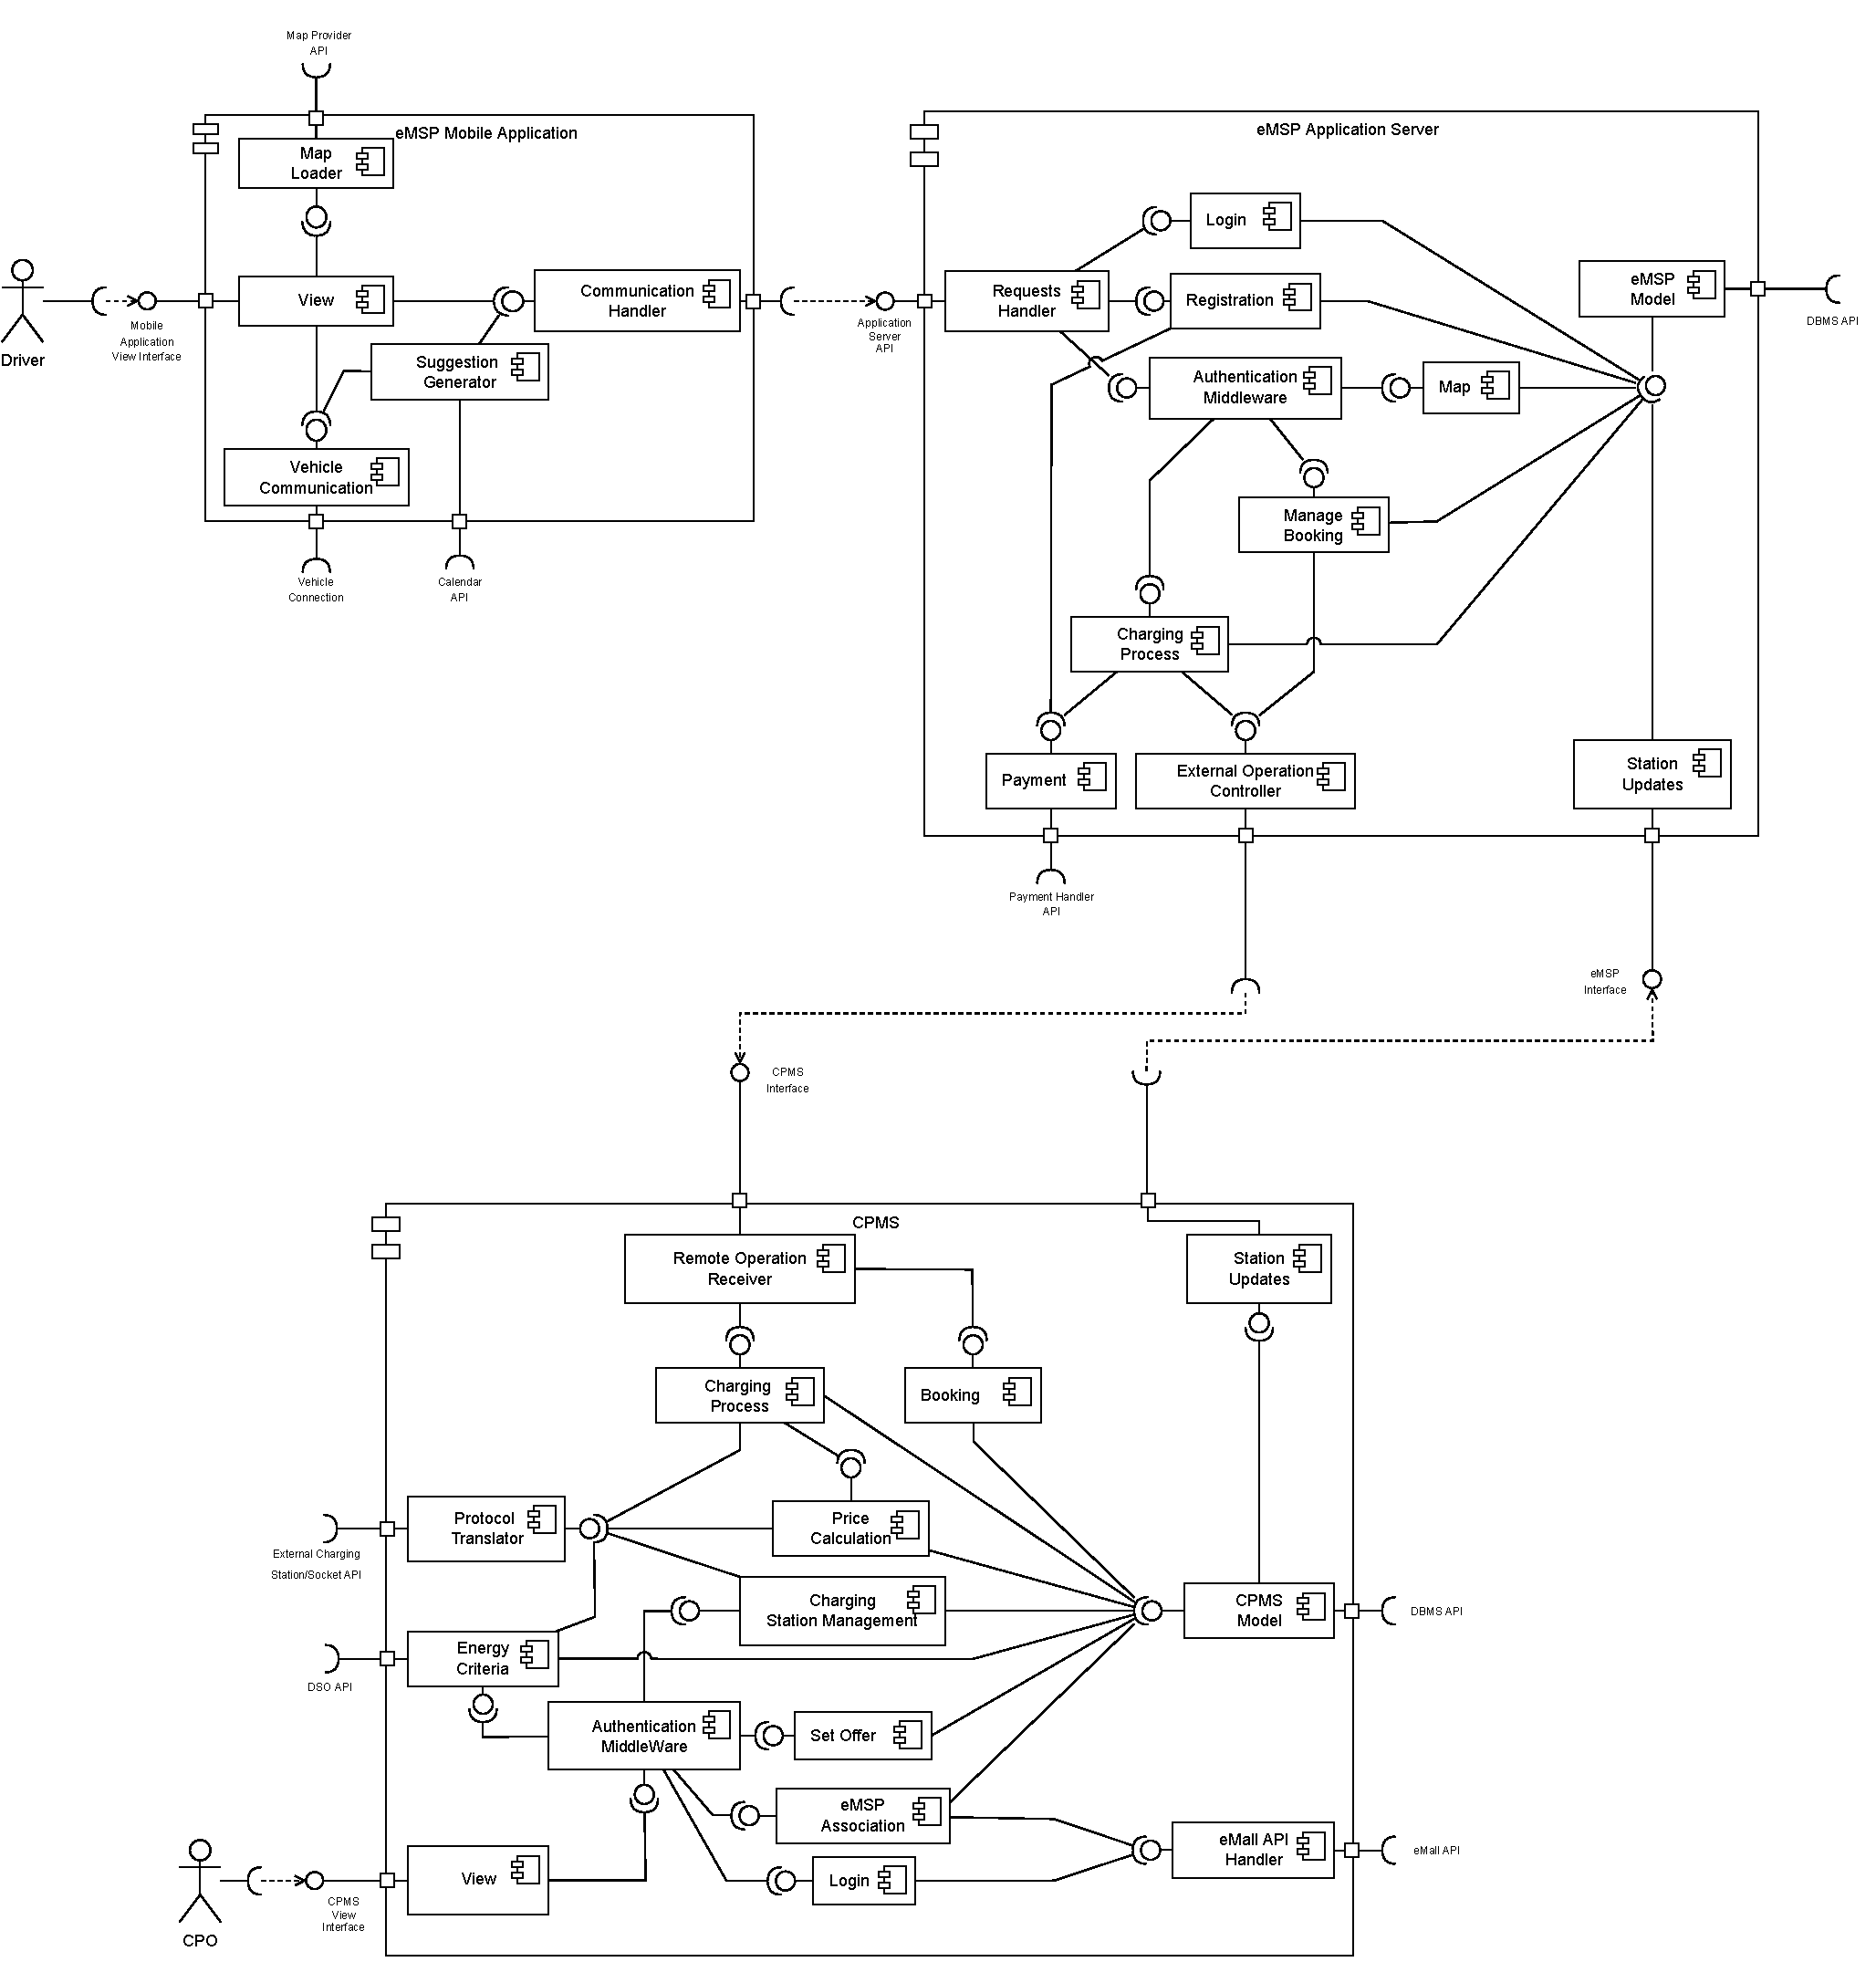
\includegraphics[
                width=1.15\textwidth,
                height=\textheight,
                keepaspectratio]{componentDiagram.pdf}
            \caption{Component Diagram}
            \label{fig:ComponentDiagram}
            \end{center}
        \end{figure}
\restoregeometry        
\subsubsection{eMSP Mobile Application}
\label{applicationView}
\paragraph{Presentation Level}
\begin{itemize}
    \item \textbf{View}: Component that will handle all the front-end rendering for the mobile application.
\end{itemize}
\paragraph{Logic Level}
\begin{itemize}
    \item \textbf{Map Loader}: Component that will handle the communication with the Maps external API.
    \item \textbf{Vehicle Communication}: Component that will handle the communication with the vehicle.
    \item \textbf{Suggestion Generator}: Component that will handle the creation of personalised suggestions for the user.
    \item \textbf{Communication Handler}: Component that will handle the communication with the eMSP Application Server.
\end{itemize}
\subsubsection{eMSP Application Server}
\label{emsPComponentView}
All components of the eMSP Application Server belong to the Logic level. 
%eMSP component diagram
\begin{itemize}
    \item \textbf{Requests Handler}: Component that will handle all the received requests.
    \item \textbf{Login}: Component that will handle the login request and authenticate a Driver.
    \item \textbf{Registration}: Component that will handle the registration requests and create a new account for a driver.
    \item \textbf{Authentication Middleware}: Component that will handle every request checking if the Driver requesting is authenticated and forwarding the request to the respective component.
    \item \textbf{Map}: Component that will handle requests for the charging stations present on the map based on their location.
    \item \textbf{Manage Booking}: Component that will handle booking requests by creating or deleting them.
    \item \textbf{Charging Process}: Component that will handle requests that need to perform operations related to a charging process.
    \item \textbf{Station Updates}: Component that will handle requests from CPMSs in order to update eMSP Model when any data related to charging stations is updated.
    \item \textbf{External Operation Controller}: Components that will handle external operation that needs communication with the CPMSs in order to be executed.
    \item \textbf{Payment}: Component that will handle communication with external payment API in order to perform money transactions.
    \item \textbf{eMSP Model}: Component that will handle communication with the DBMS.
\end{itemize}
\subsubsection{CPMS}
%CPMS component diagram
\begin{itemize}
    \item \textbf{View}: Component that will handle all the front-end rendering for the CPMS application.
    \item \textbf{Authentication Middleware}: Component that will handle every request checking if the CPO requesting is authenticated and forwarding the request to the respective component.
    \item \textbf{Energy Criteria}: Component that will handle the modification and update of both energy acquisition and revenue criteria.
    \item \textbf{Login}: Component that will handle the login request and authenticate a CPO.
    \item \textbf{eMSP Association}: Component that will handle the association process between the CPMS and eMSPs.
    \item \textbf{Set Offer}: Component that will handle the requests of setting offers by the CPO.
    \item \textbf{eMall API Handler}: Component that will handle the communication with the eMall API
    \item \textbf{Price Calculation}: Component that will calculate the price after a charging process ends.
    \item \textbf{Charging Station Management}: Component that will handle the requests of charging station management by the CPO.
    \item \textbf{Protocol Translator}: Component that will handle communication with charging stations API and charging sockets API
    \item \textbf{Remote Operation Receiver}: Components that will handle external requests from the eMSP.
    \item \textbf{Booking}: Component that will handle the booking process for a charging station.
    \item \textbf{Charging Process}: Component that will handle the charging process for a charging station.
    \item \textbf{Station Update}: Component that will perform requests to associated eMSPs in order to update them when any data related to charging stations is updated.
    \item \textbf{CPMS Model}: Component that will handle the communication with the DBMS.
\end{itemize}
\label{CPMSComponentView}
\newpage
\subsubsection{eMSP Model ER Diagram}
The following ER diagram displays a detailed view of a possible internal structure of the \textit{eMSP Model} component.
\begin{figure}[H]
    \begin{center}
    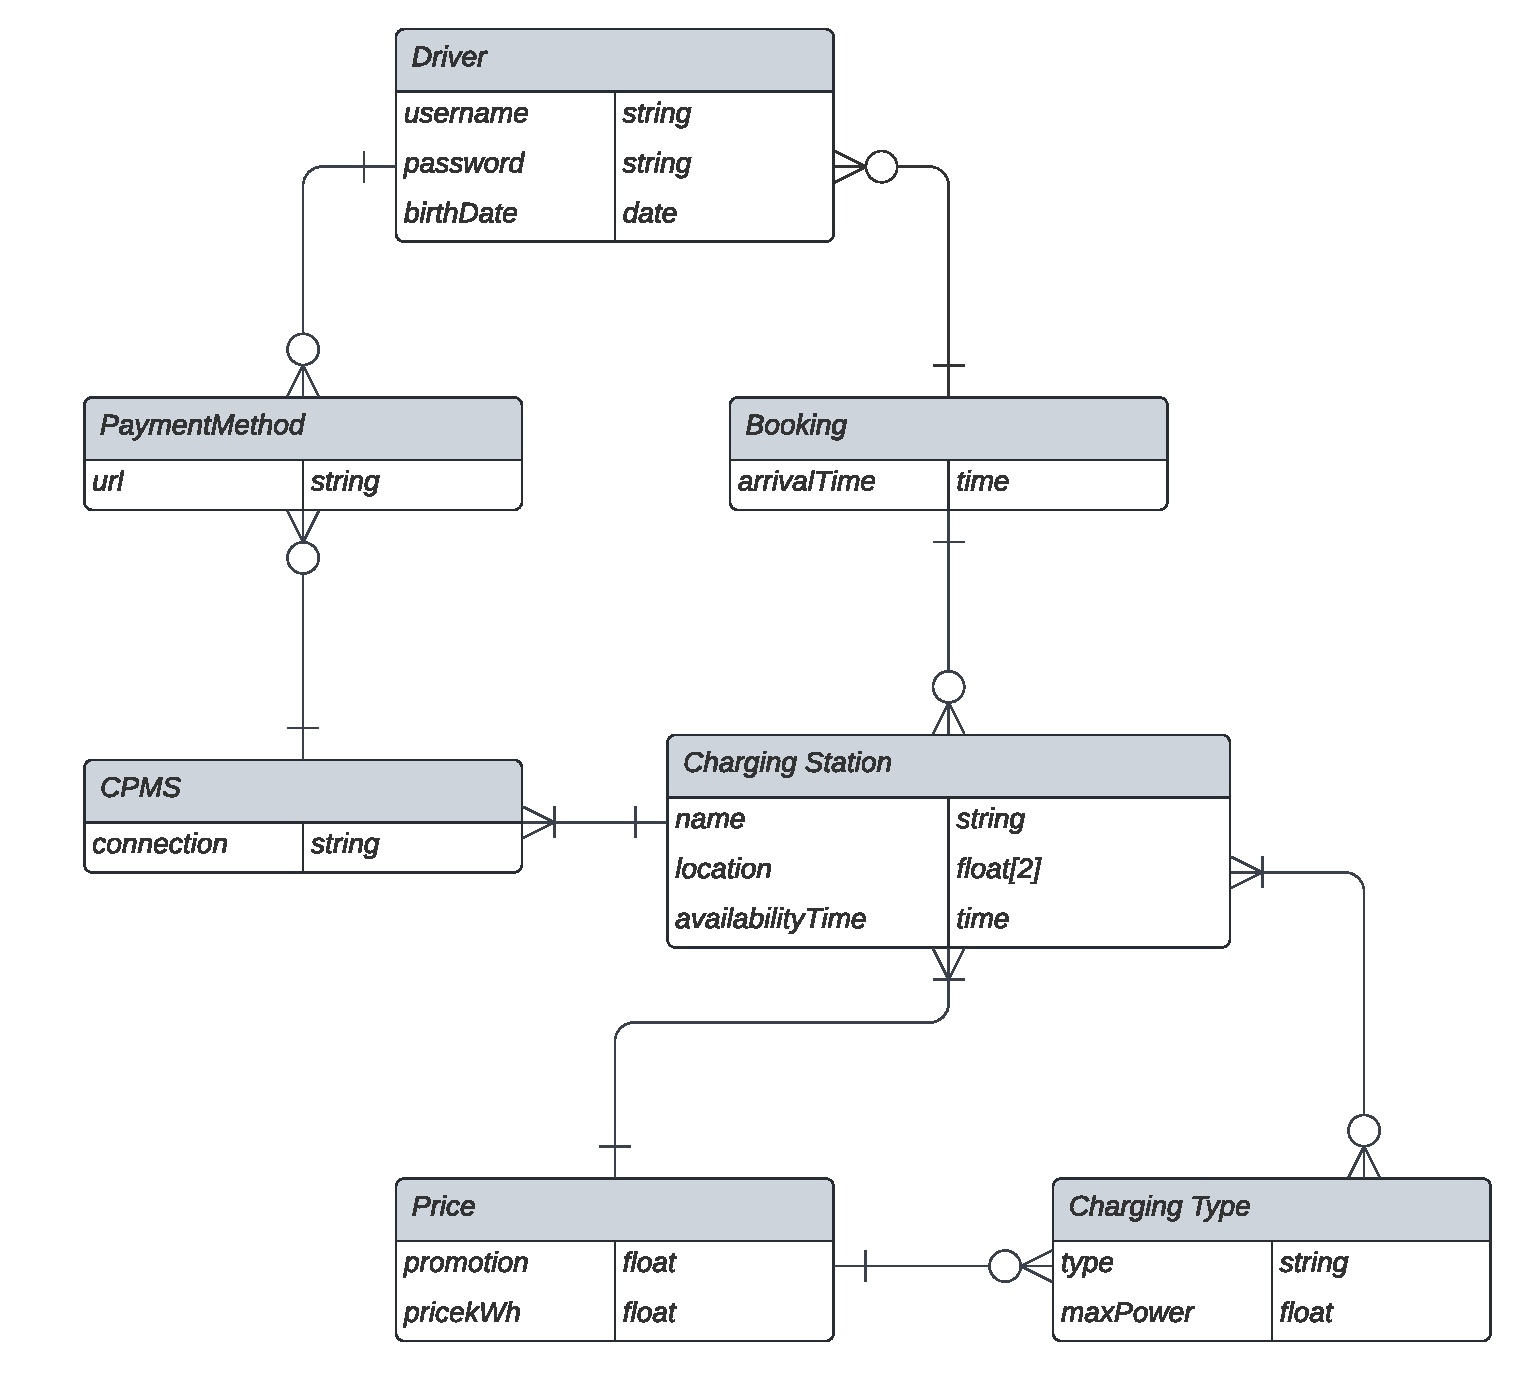
\includegraphics[
        width=\textwidth,
        height=\textheight,
        keepaspectratio]{ER/eMSP ER Diagram.pdf}
    \caption{eMSP Model ER Diagram}
    \label{fig:eMSPERDiagram}
    \end{center}
\end{figure}
\newpage
\subsubsection{CPMS Model ER Diagram}
The following ER diagram displays a detailed view of a possible internal structure of the \textit{CPMS Model} component.
\begin{figure}[H]
    \begin{center}
    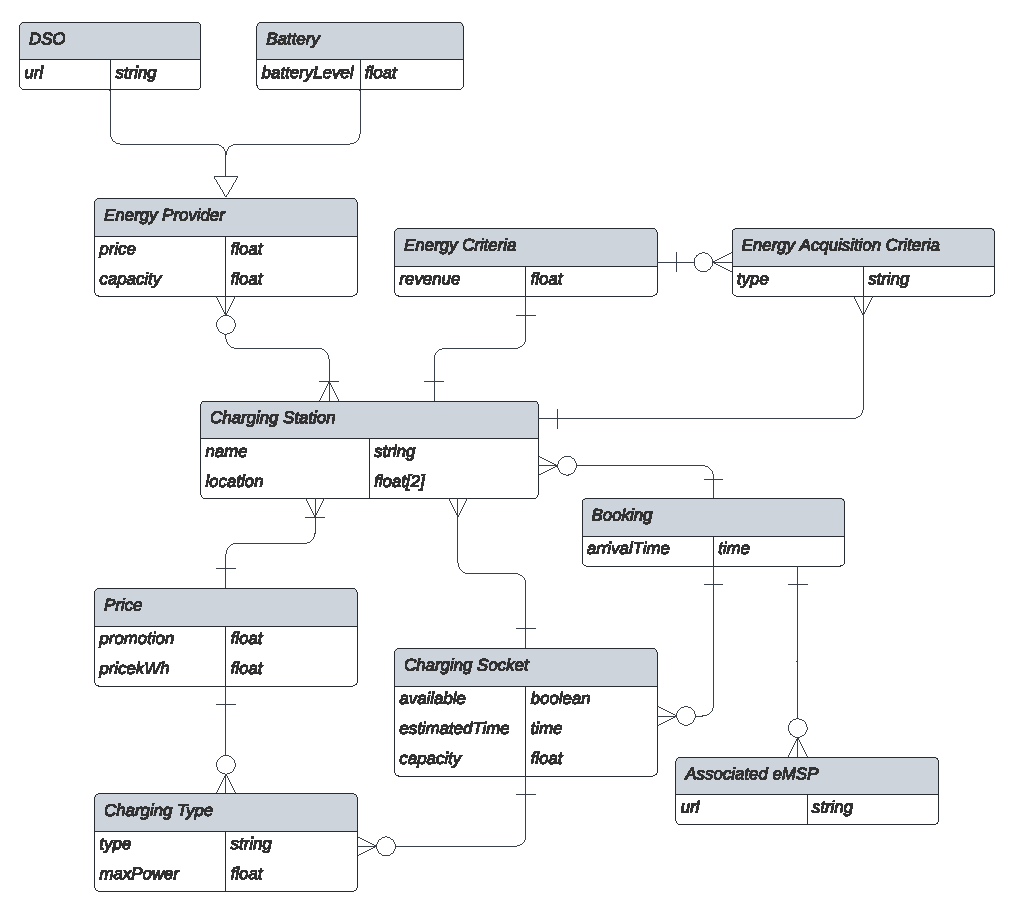
\includegraphics[
        width=\textwidth,
        height=\textheight,
        keepaspectratio]{ER/CPMS ER Diagram.pdf}
    \caption{CPMS Model ER Diagram}
    \label{fig:CPMSERDiagram}
    \end{center}
\end{figure}
%\begin{itemize}
 % \item \textbf{} contains the activities  as well as the Java code.
 % \item \textbf{gen}
 % \item \textbf{assets}
 % \item \textbf{bin}
%\end{itemize}
\newpage
\section{Deployment View}
\label{sec:deploymentView}
The following deployment diagram shows the execution architectures of the systems. It specifies the hardware and software environments as well as middlewares present and protocols needed to communicate between the systems.
\begin{figure}[H]
            \begin{center}
            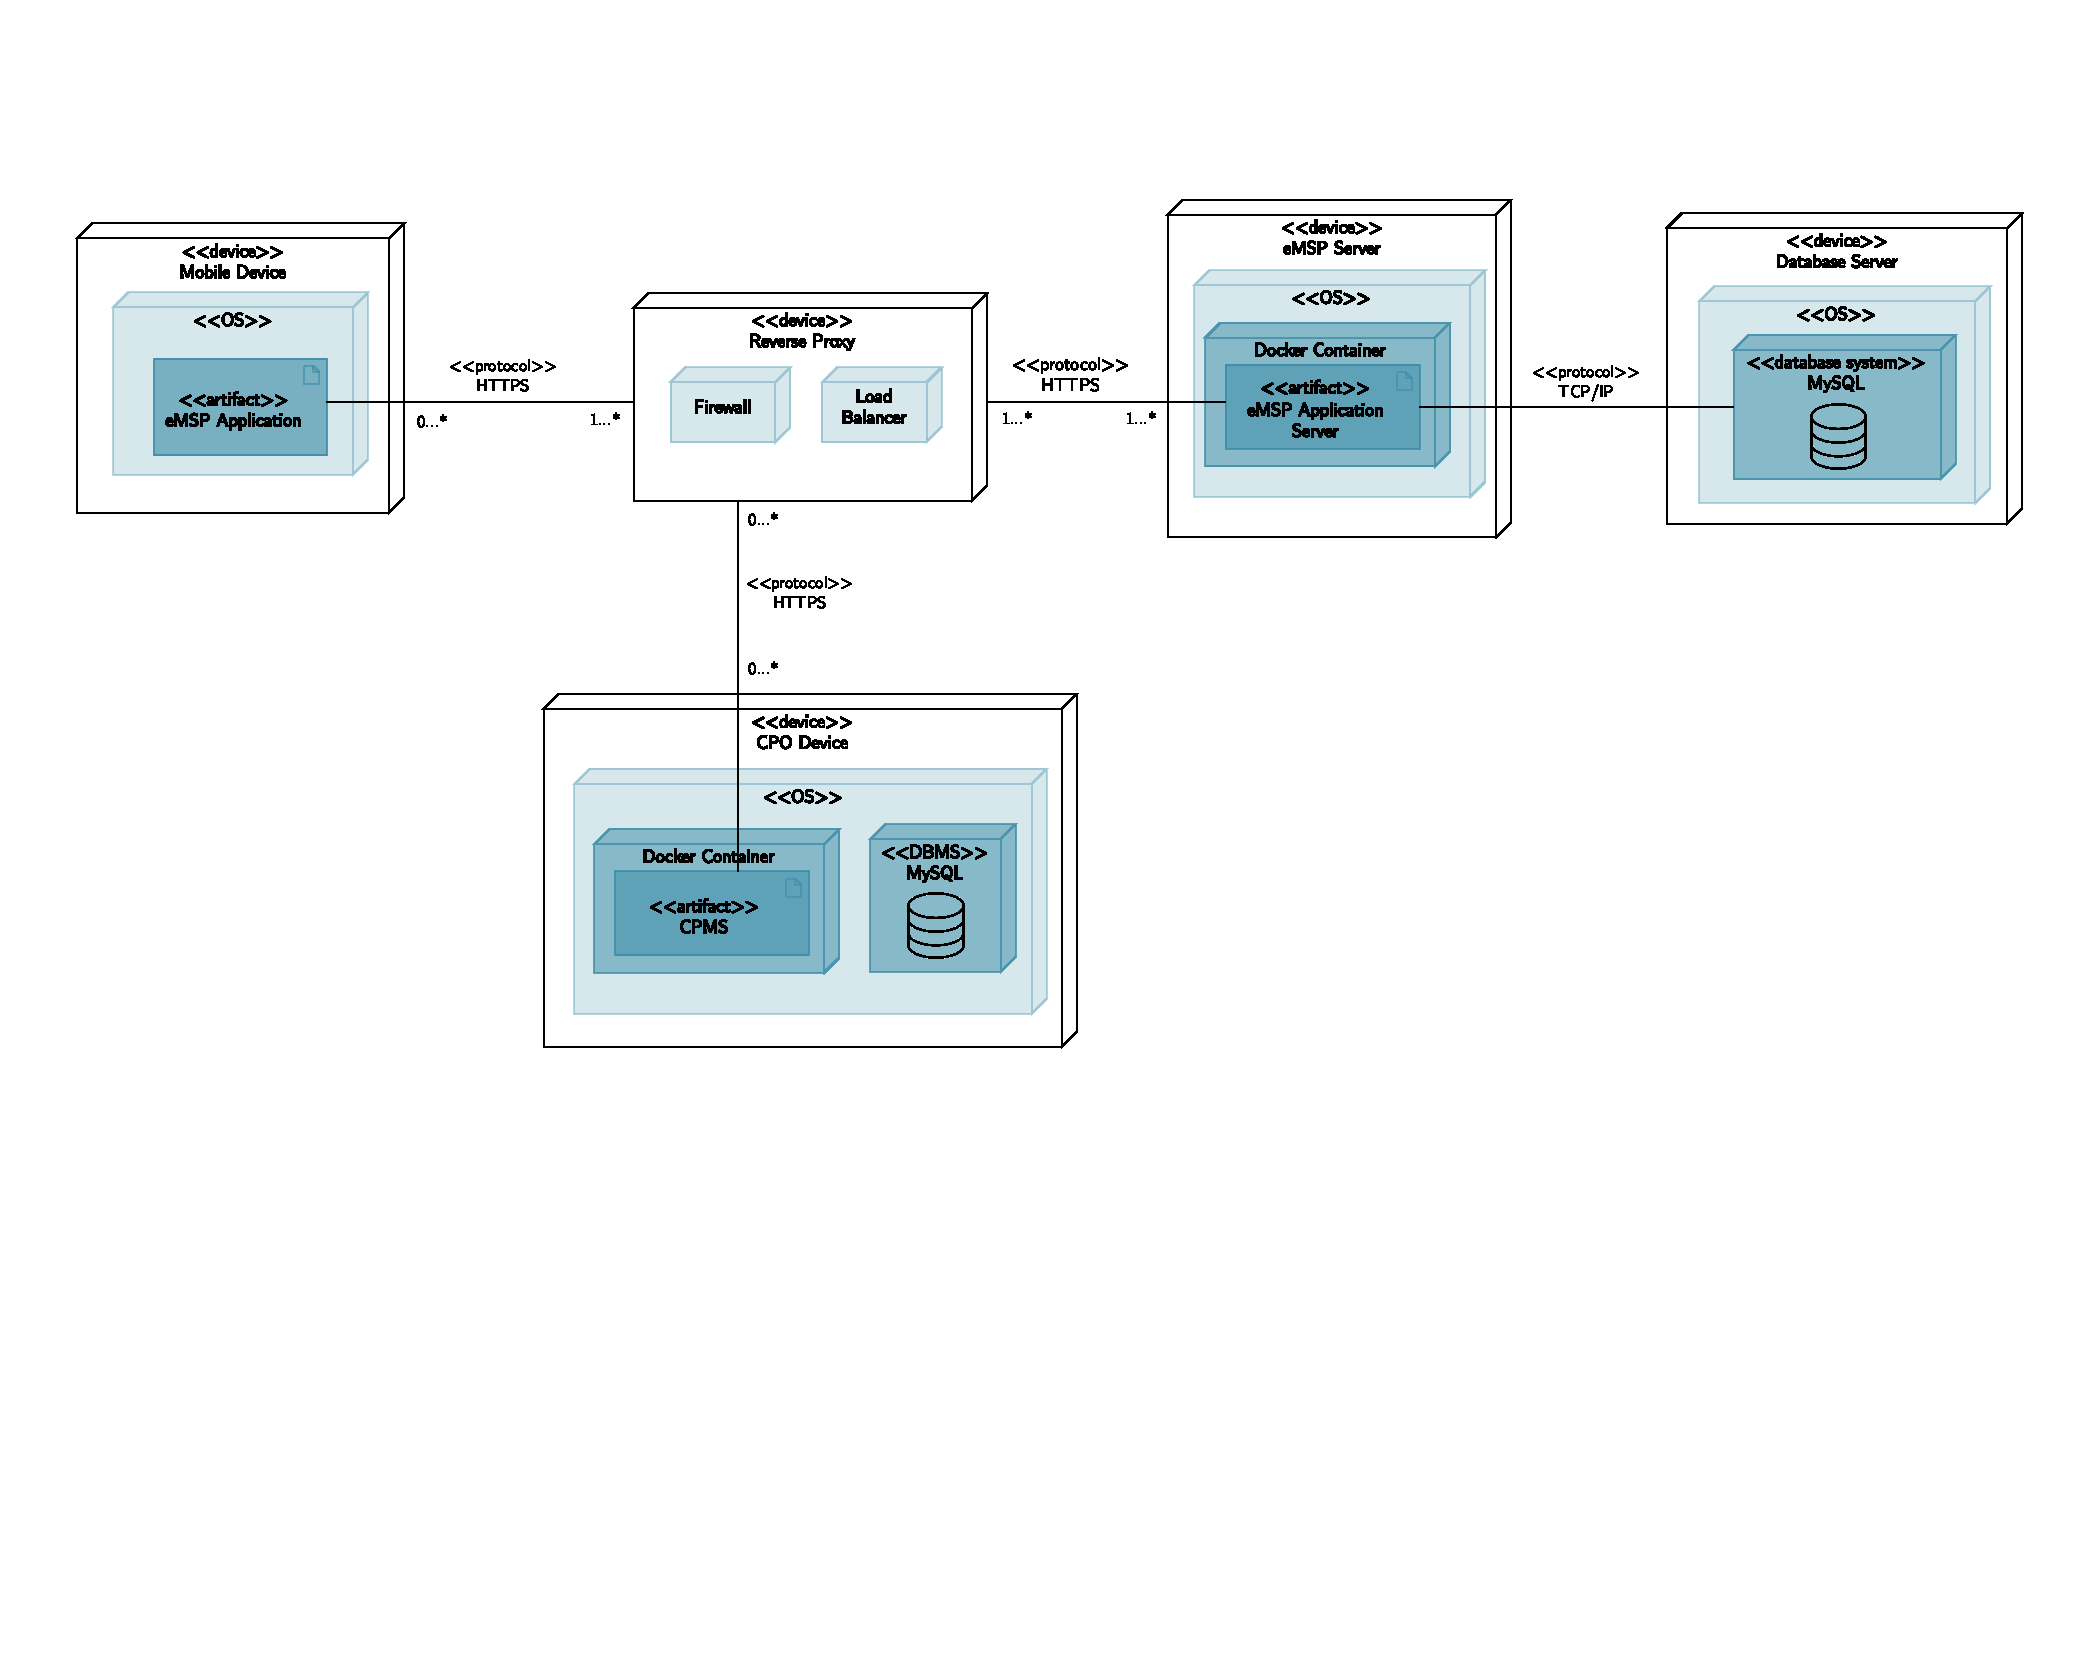
\includegraphics[
                width=\textwidth,
                height=\textheight,
                keepaspectratio]{deploymentDiagram.pdf}
            \caption{Deployment Diagram}
            \label{fig:DeploymentDiagram}
            \end{center}
        \end{figure}
\begin{itemize}
    \item \textbf{Mobile Device: }Personal device with internet access used by the Driver to run the eMSP Application.
    \item \textbf{Reverse Proxy: }The reverse proxy acts as a single point of contact for users, protecting the application servers behind it from malicious traffic using a firewall. It also includes a load balancer, which distributes incoming requests evenly across the application servers to improve performance, availability and reliability. Multiple reverse proxies can be deployed in different locations to increase availability.
    \item \textbf{eMSP Server: }The application server hosts the eMSP's application logic and interacts with the database server. Using multiple application servers can improve reliability and availability and allow the system to handle a larger number of concurrent requests.
    \item \textbf{Database Server: }The database server, which includes a database management system (DBMS), will host the database. Using multiple database servers can improve reliability and increase the availability of the eMSP.
    \item \textbf{CPO Device: }The CPO uses a personal device with internet access to run the CPMS application. In order to receive external requests from eMSPs through the internet, the device must also have a firewall to protect against potential security threats.
    
\end{itemize}
\section{Runtime View}
\label{sec:runtimeView}
The following sequence diagrams depict the behaviour of the key components of the eMSP and the CPMS subsystems. These diagrams provide a high-level overview of the interaction between the various components. Further details and implementation will be addressed during the development process.
\subsection{Sequence Diagrams}
\label{subsec:sequenceDiagrams}
A detail that should be noticed in the following sequence diagram, is the async request made by the \textit{View} (Both for the eMSP and the CPMS). This is needed in order to let the driver have a responsive and fluid user interface. 
\begin{enumerate}
    
    \item \textbf{Driver Authentication Check}
        \begin{figure}[H]
            \begin{center}
            \includegraphics[
                width=0.96\textwidth,
                height=0.96\textheight,
                keepaspectratio]{SeqDia/Driver_Authentication_check}
            \caption{Authentication of a Driver}
            \label{fig:DriverAuth}
            \end{center}
        \end{figure}
        The figure illustrates the process of authenticating a Driver for every request, except for login and registration. The \textit{Specific Component} in the figure refers to the component capable of responding to the Driver's request. If the driver is not authenticated, their mobile application will be redirected to the login view. To implement the isLogged(session) function in the sequence diagram and create a session to identify the Driver, it is recommended to use a technology like JWT, which avoids the need to query the DBMS.[\ref{jwt}]\\
        
        \newpage
        \item \textbf{Driver Registration}
        \begin{figure}[H]
            \begin{center}
            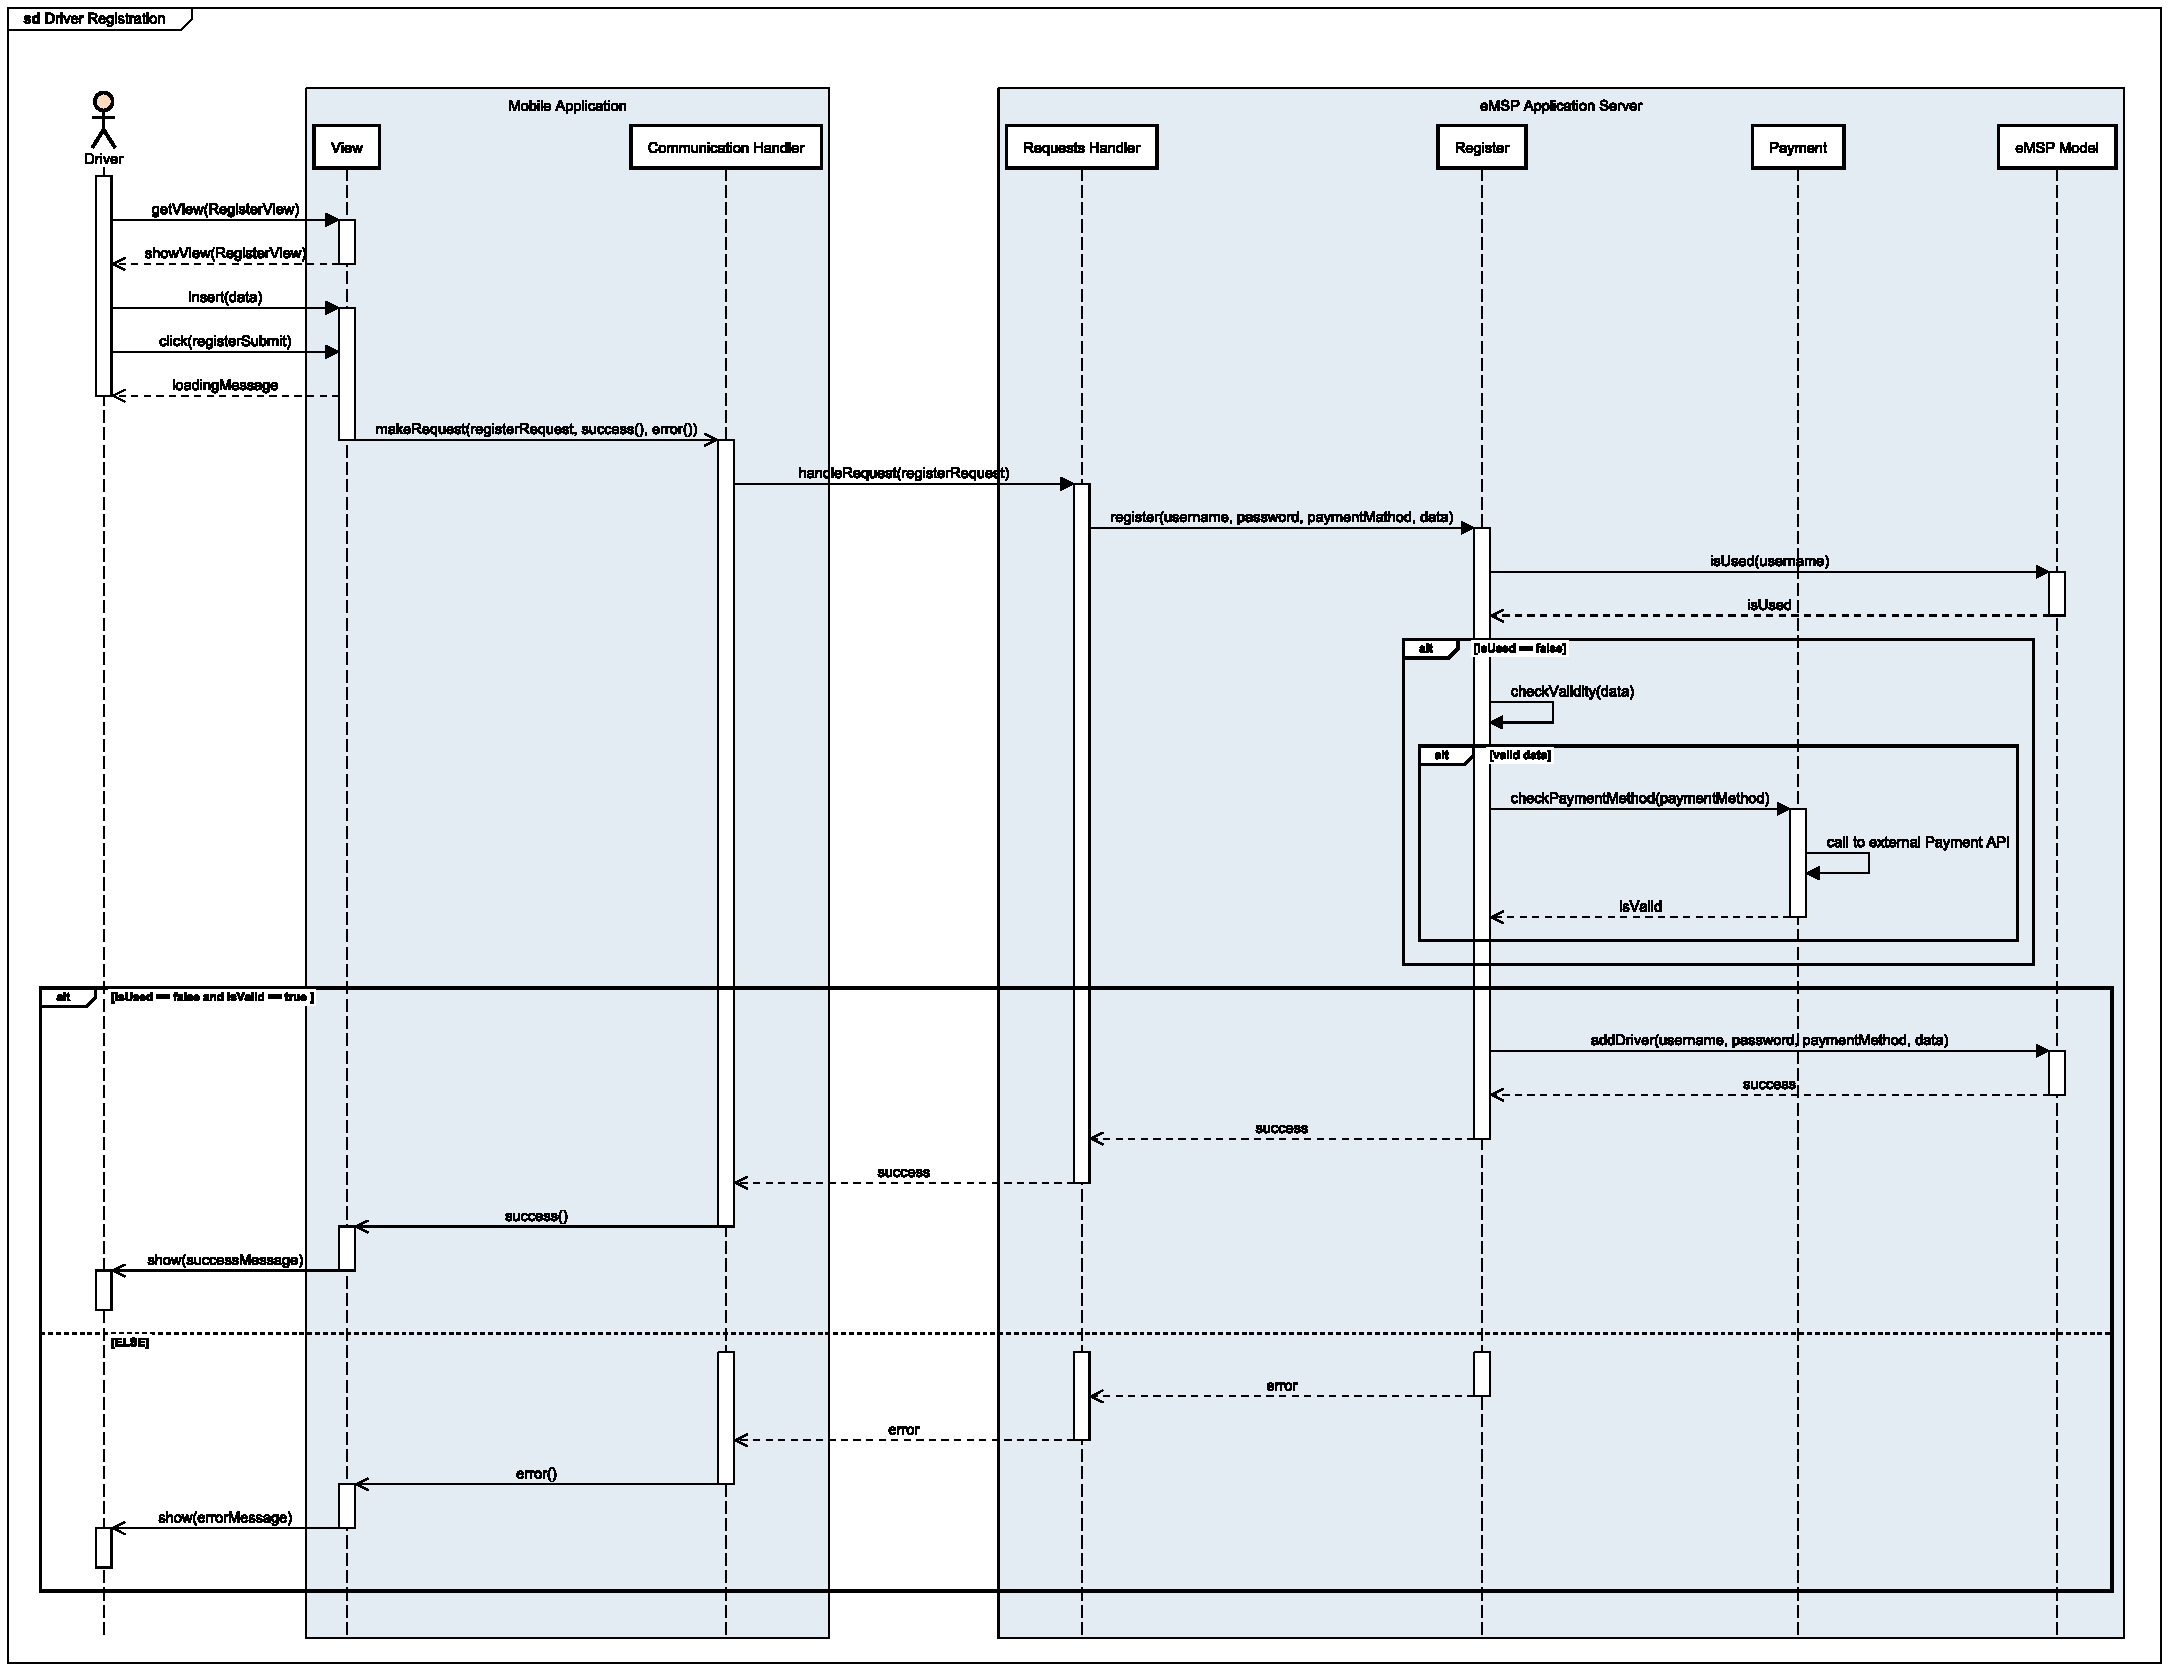
\includegraphics[
                width=\textwidth,
                height=\textheight,
                keepaspectratio]{SeqDia/Driver_Registration}
            \caption{Registration of a Driver}
            \label{fig:DriverRegistration}
            \end{center}
        \end{figure}
        The figure shows the process of the creation of a new account for a Driver. In particular, if the Driver wants to register himself on the platform, he should insert a valid payment method and credentials otherwise, the process will fail.
        \newpage
        \item \textbf{Driver Login}
        \begin{figure}[H]
            \begin{center}
            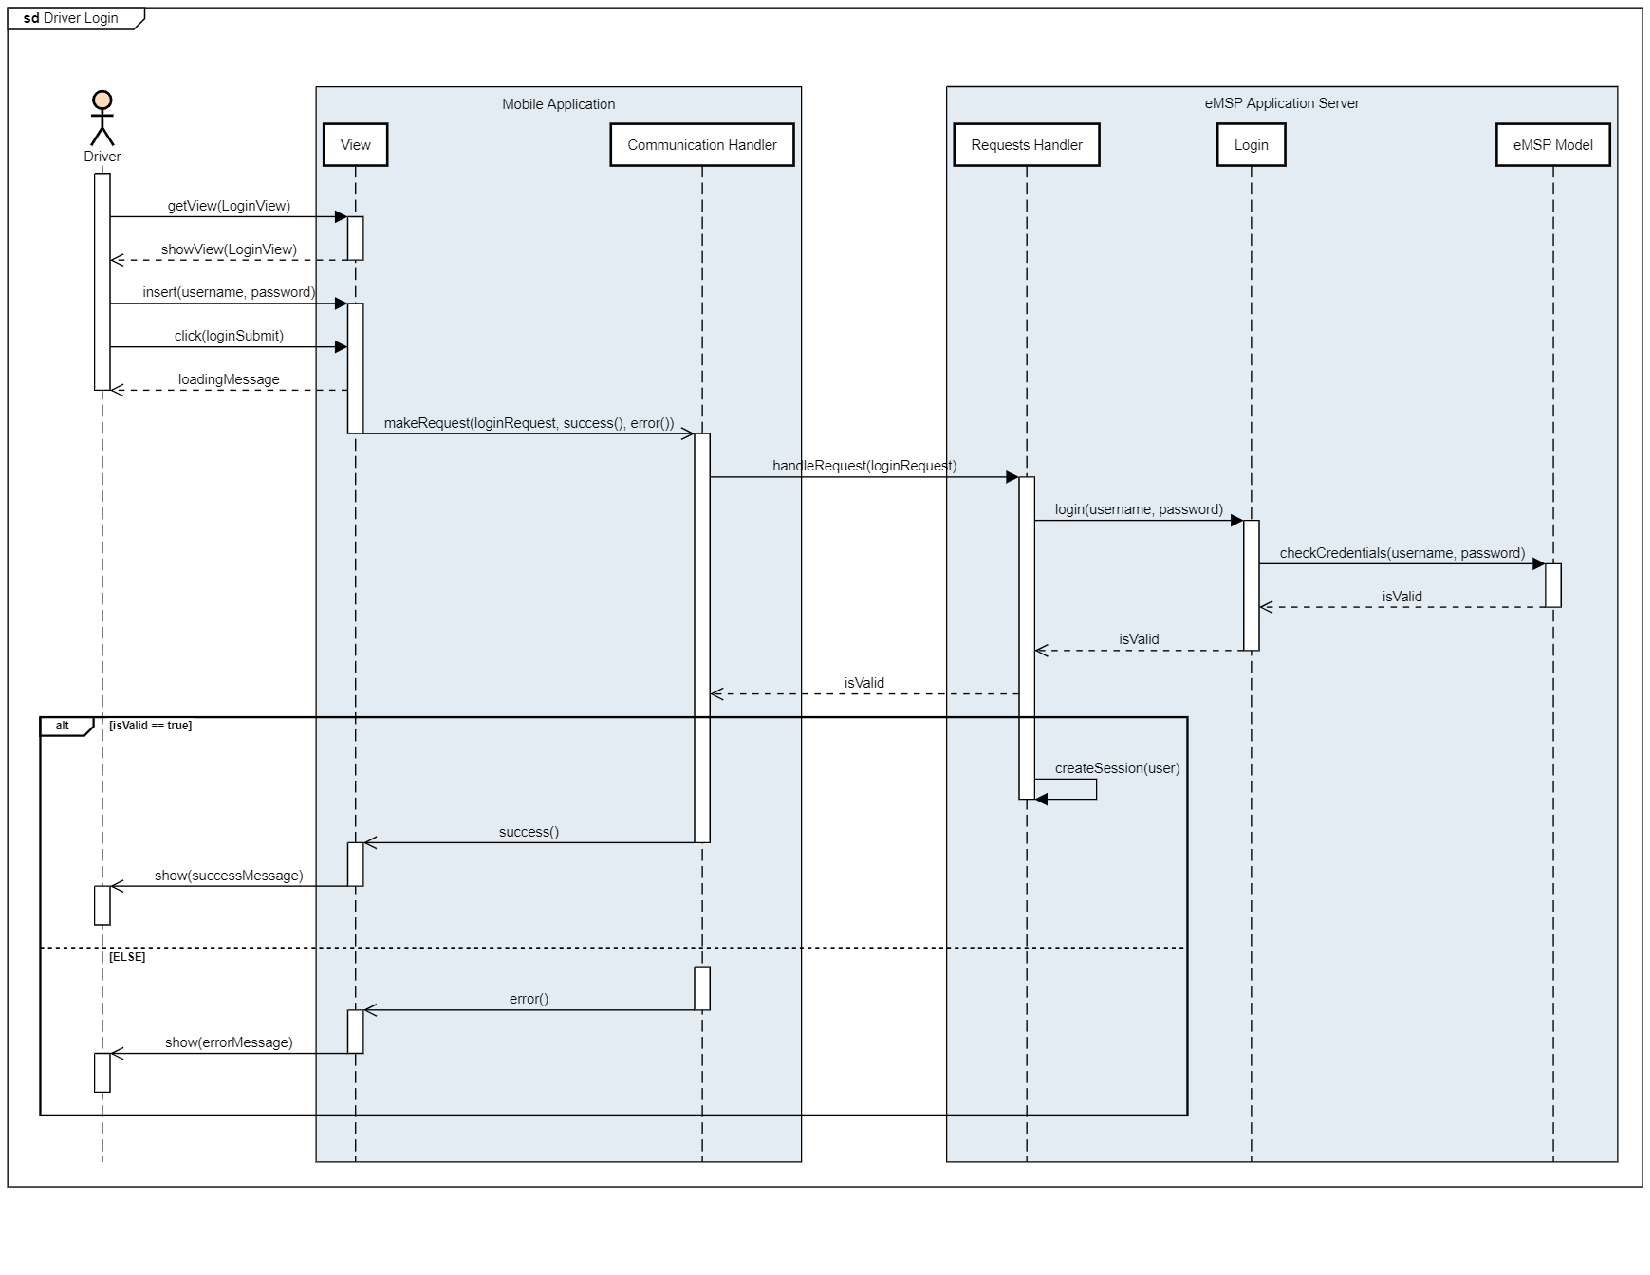
\includegraphics[
                width=\textwidth,
                height=\textheight,
                keepaspectratio]{SeqDia/Driver_Login}
            \caption{Login of a Driver}
            \label{fig:DriverLogin}
            \end{center}
        \end{figure}
        The figure shows the process of login. As aforementioned, after login, the platform should create a session in order to let the Driver stay authenticated. This session should provide basic information about the Driver such as his ID number. \ref{jwt}
        \newpage
        \item \textbf{Check Map}
        \begin{figure}[H]
            \begin{center}
            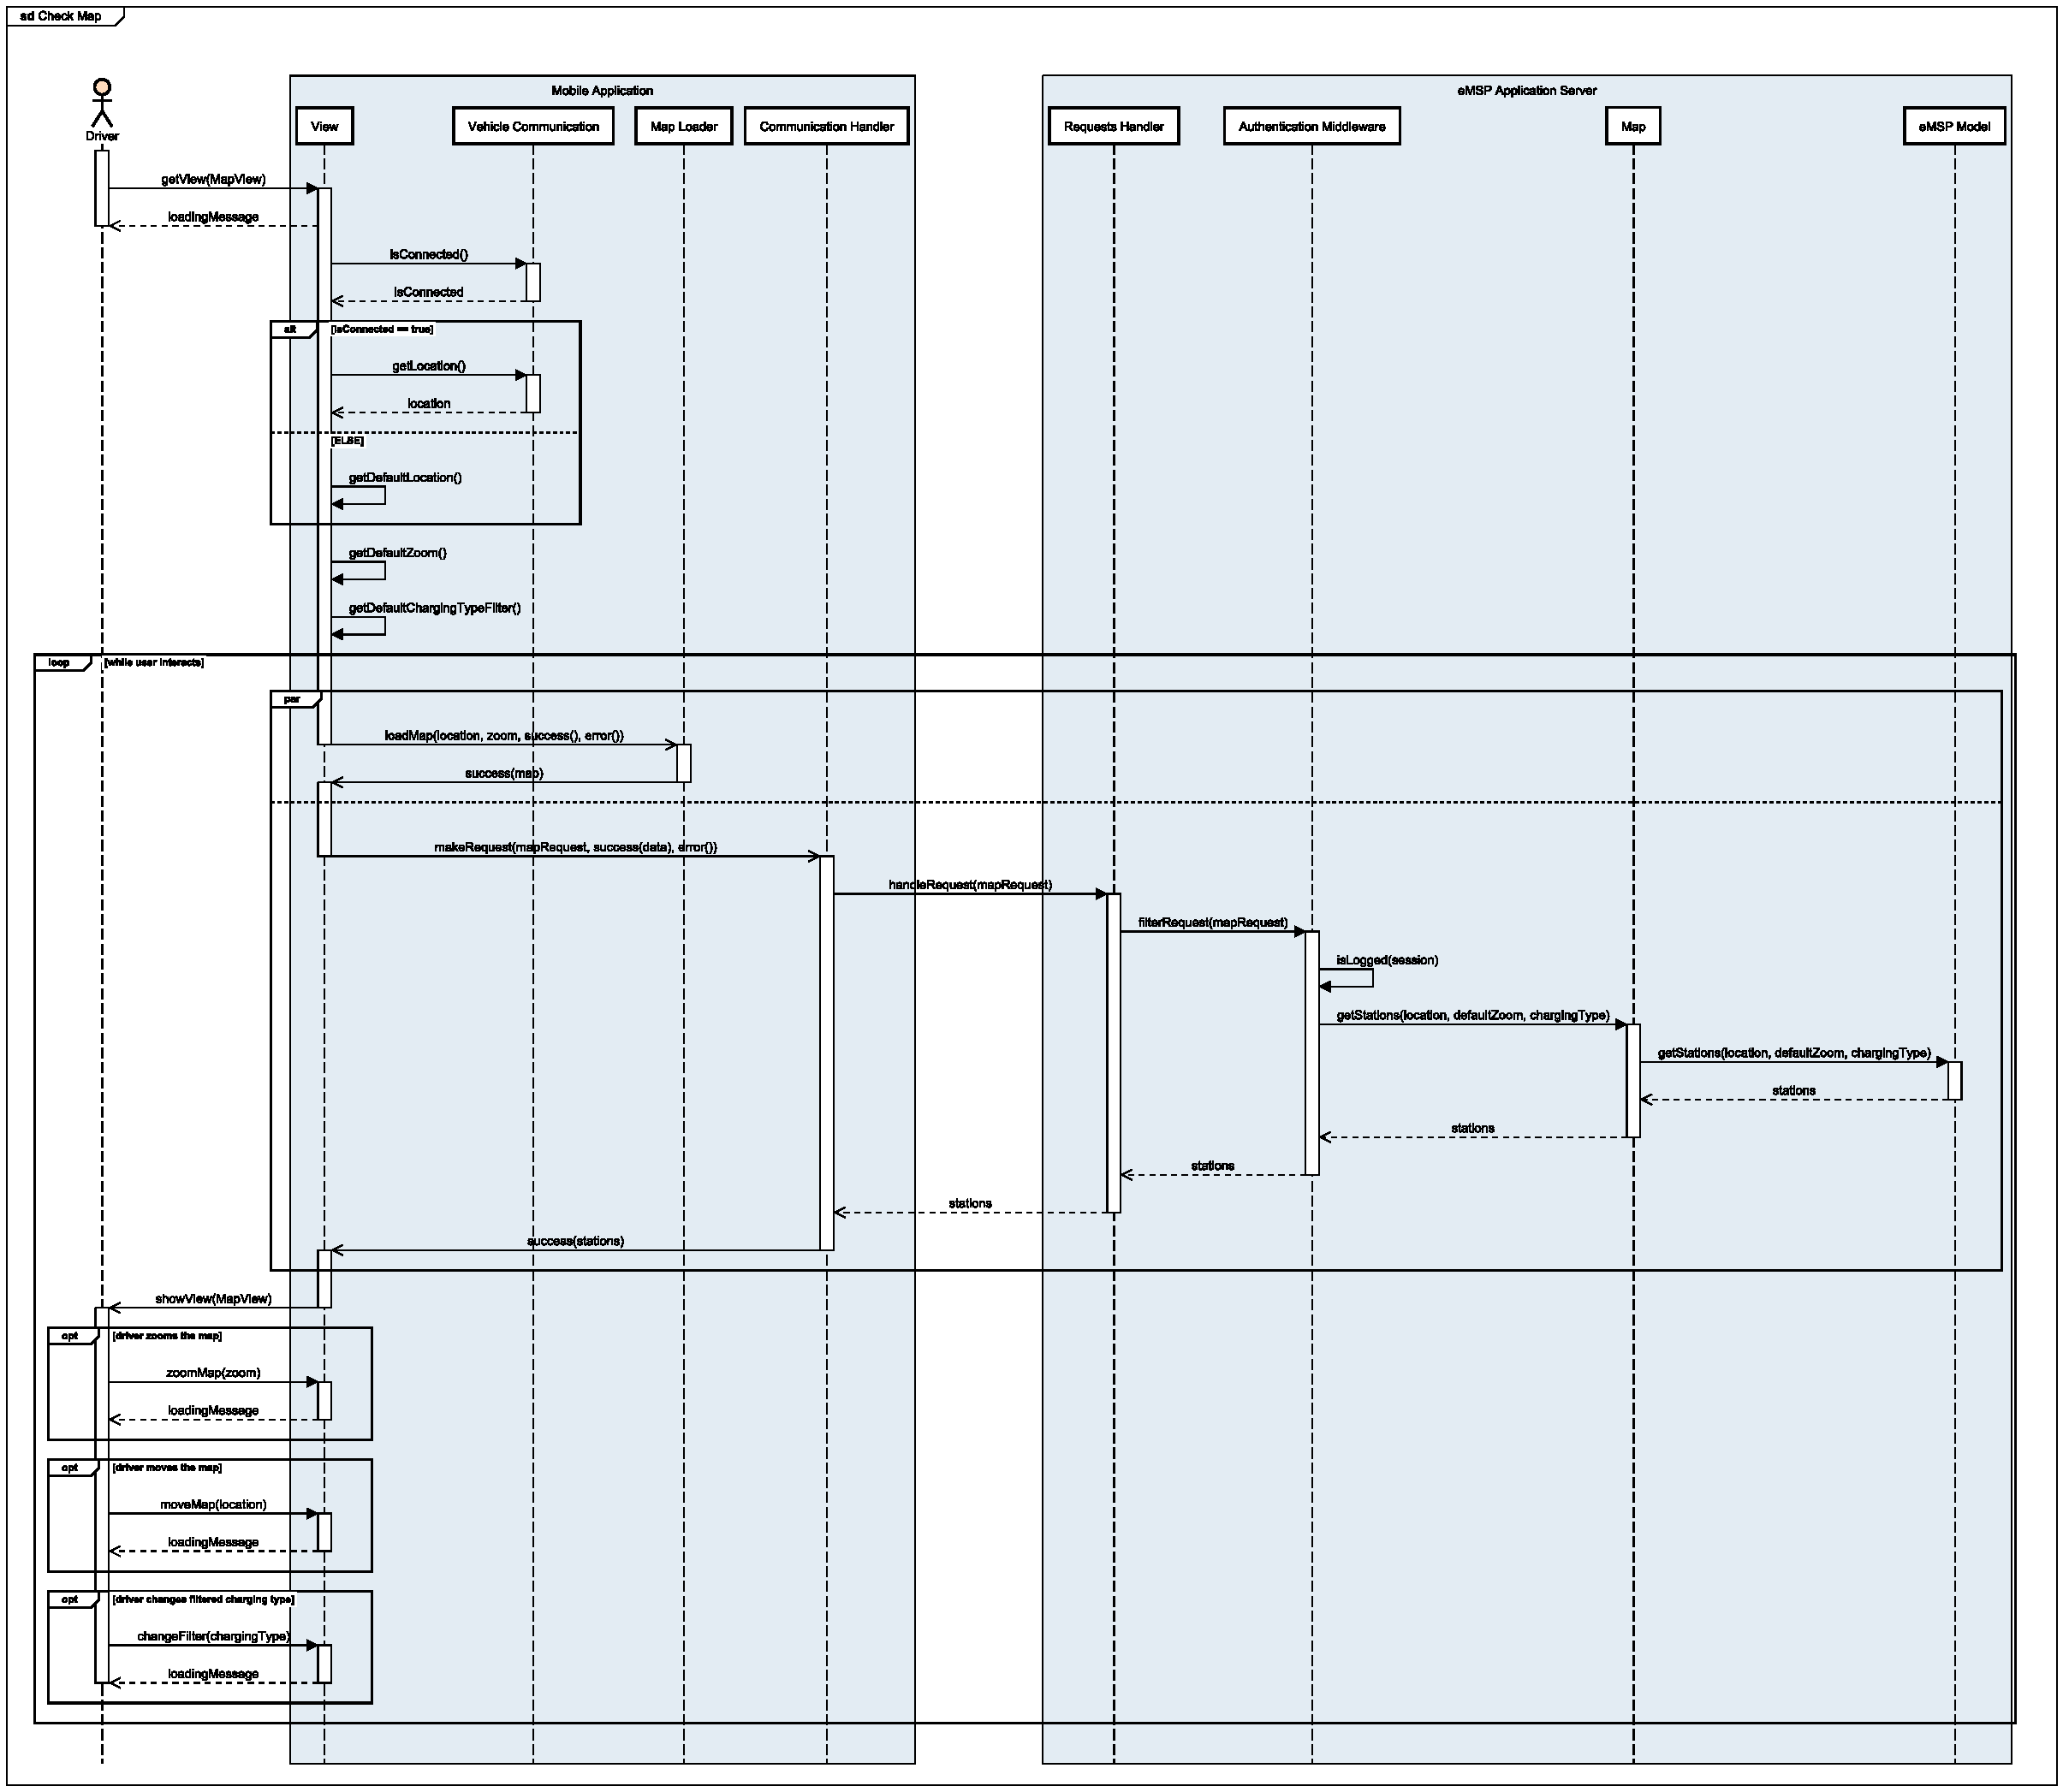
\includegraphics[
                width=\textwidth,
                height=\textheight,
                keepaspectratio]{SeqDia/Check_Map}
            \caption{Driver interacts with map}
            \label{fig:CheckMap}
            \end{center}
        \end{figure}
        The figure shows the process of the Driver checking the map and charging station present. If he is connected with his vehicle the application will show the charging station nearby his vehicle otherwise it will show a default location with default zoom and default charging type filter. (This can be decided during implementation). Every time one of the previous parameters is changed the app will ask the server for the data related to the parameters.
        \newpage
        \item \textbf{Check Station Info}
        \begin{figure}[H]
            \begin{center}
            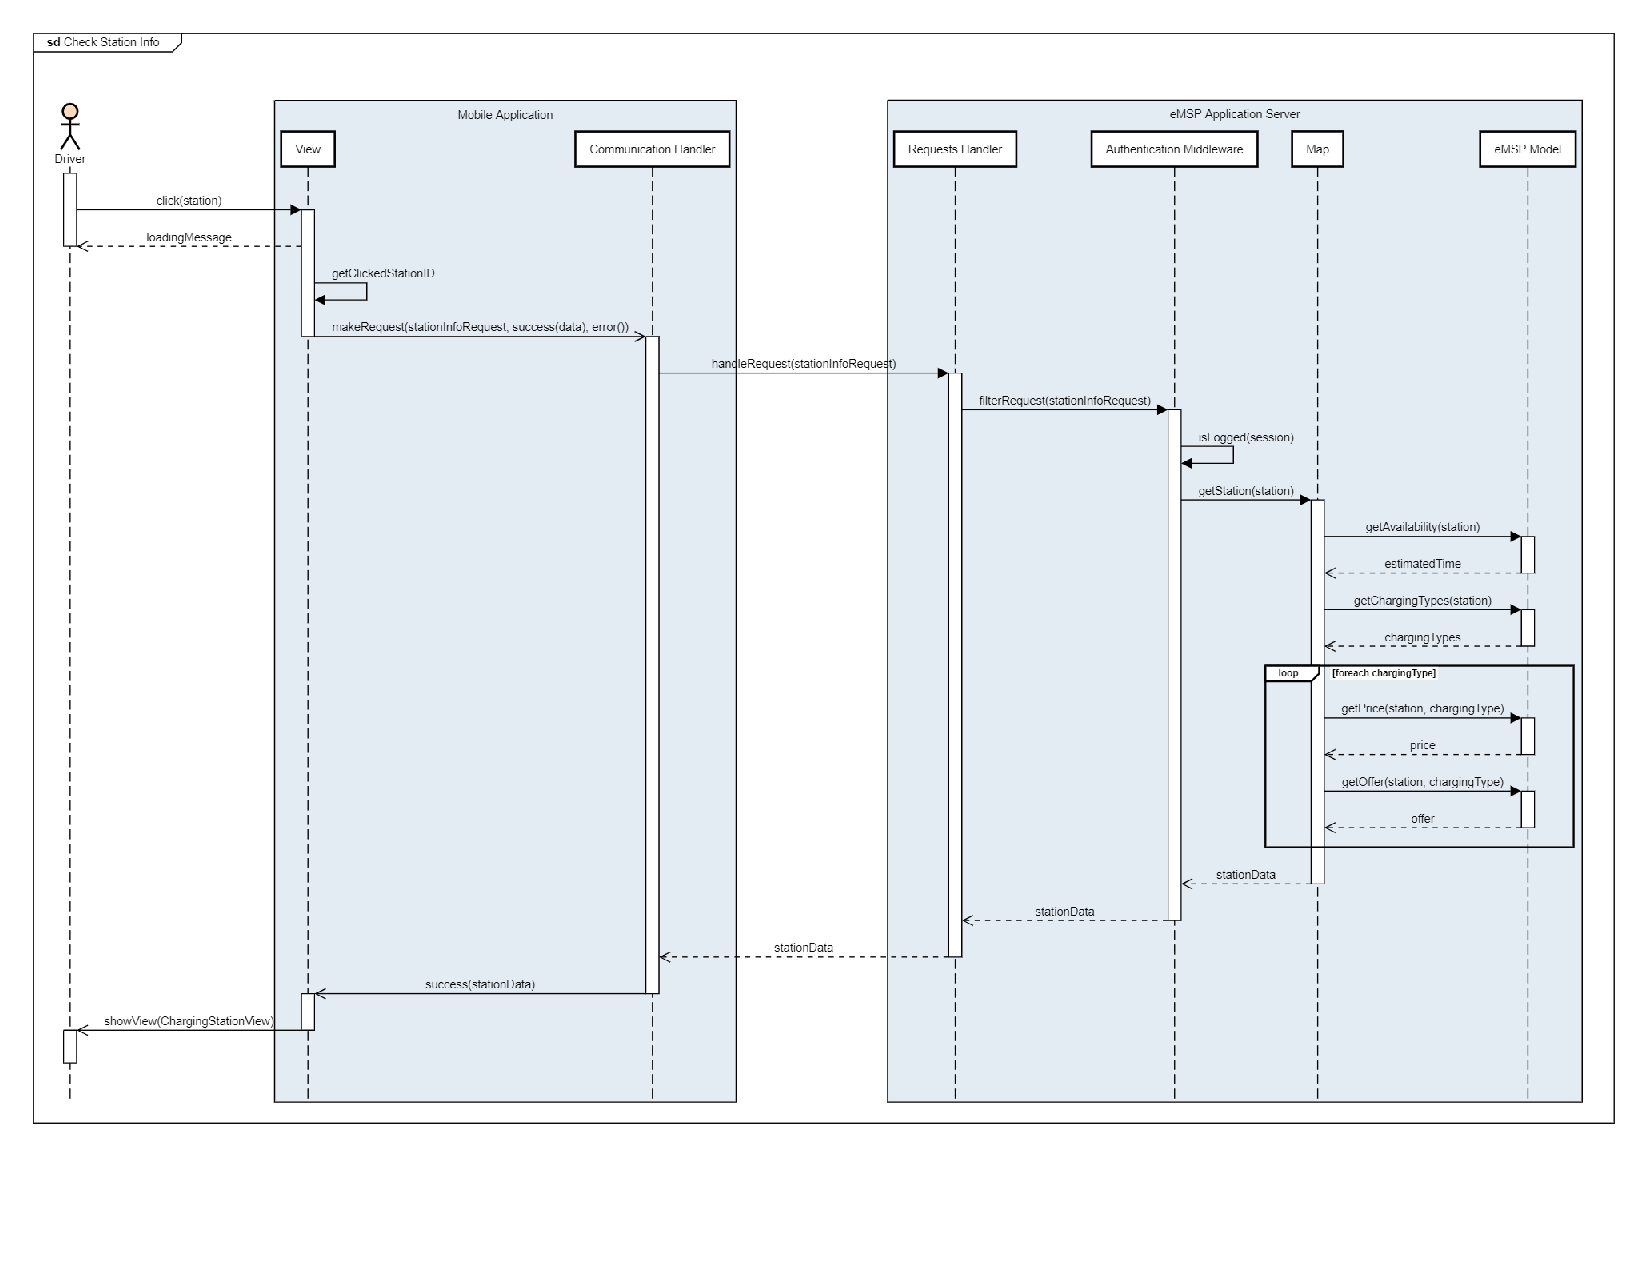
\includegraphics[
                width=\textwidth,
                height=\textheight,
                keepaspectratio]{SeqDia/Check_Station_Info}
            \caption{Driver checks a station's info}
            \label{fig:CheckStationInfo}
            \end{center}
        \end{figure}
        The figure shows the process of a Driver checking station info such as his availability, charging types and offers.
        \newpage
        \item \textbf{Create Booking}
        \begin{figure}[H]
            \begin{center}
            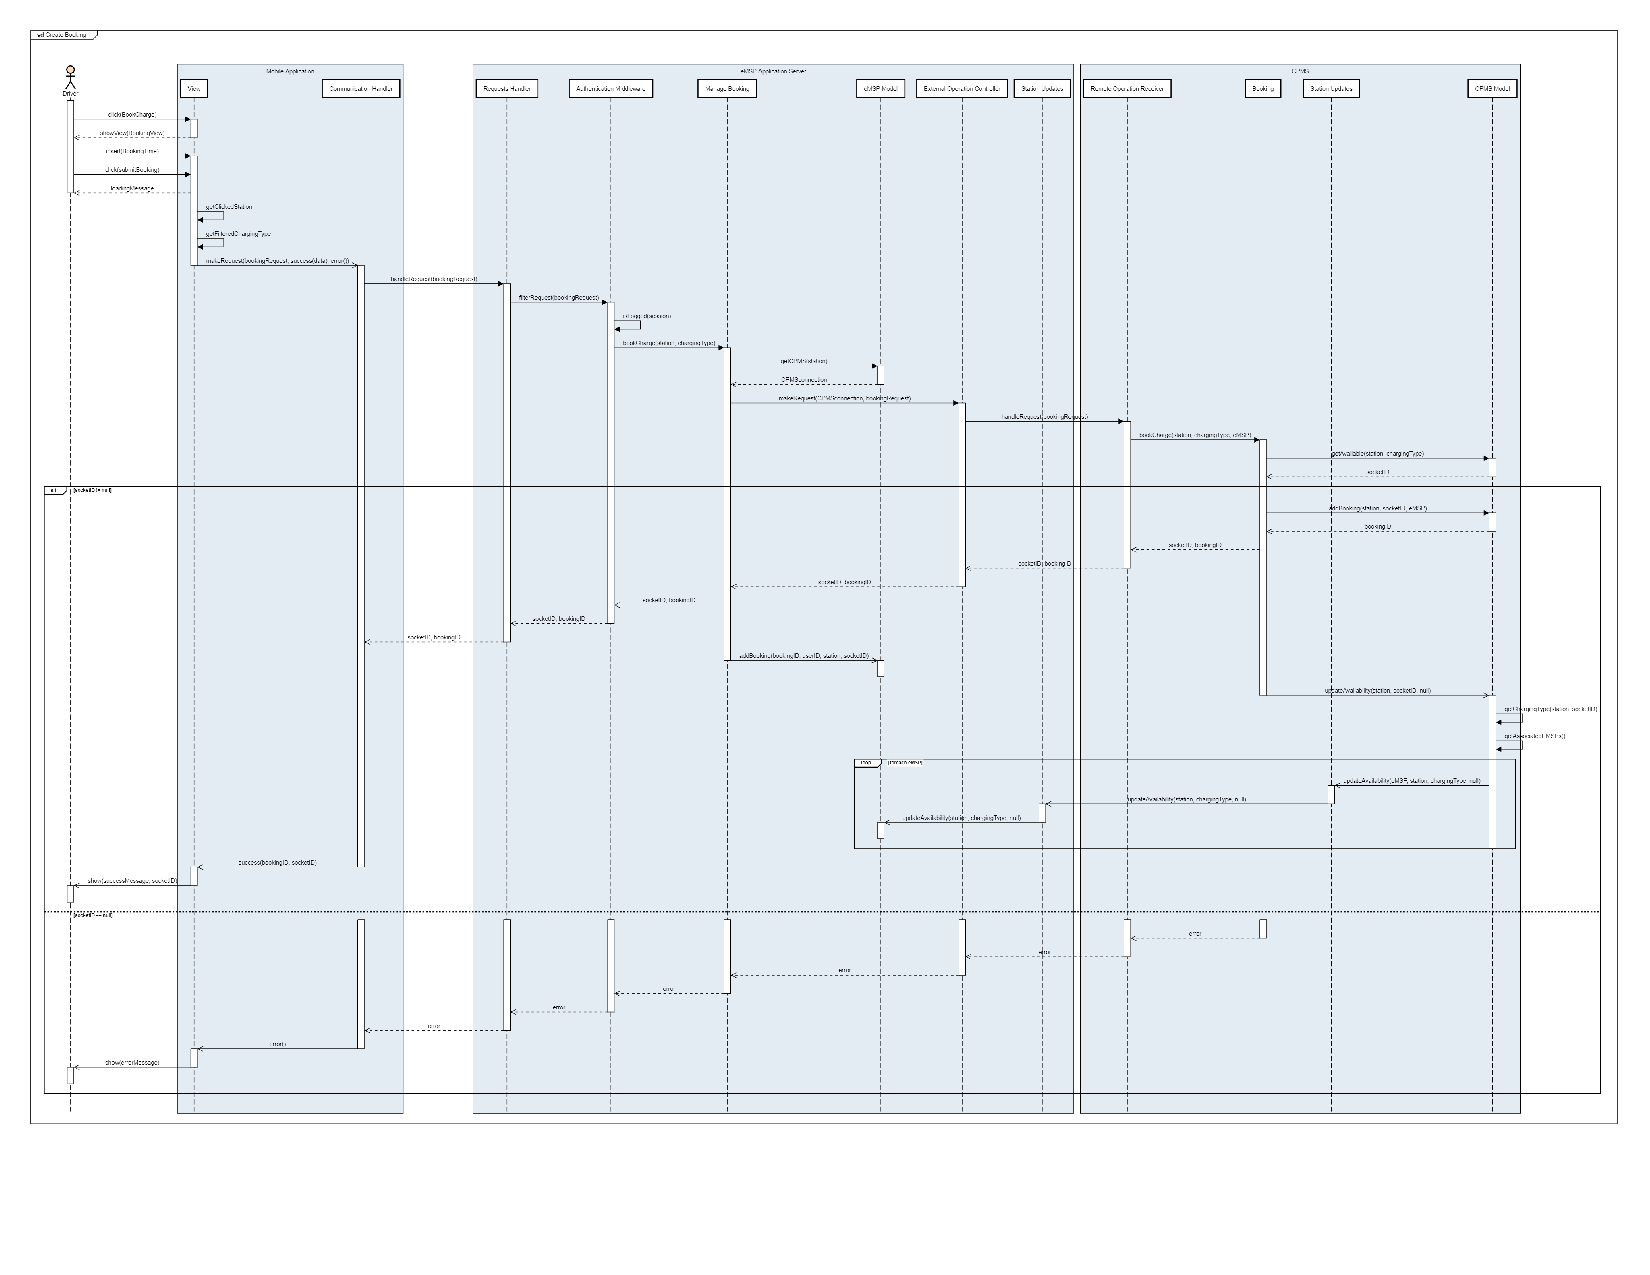
\includegraphics[
                width=\textwidth,
                height=\textheight,
                keepaspectratio]{SeqDia/Create_Booking}
            \caption{Driver creates a booking}
            \label{fig:CreateBooking}
            \end{center}
        \end{figure}
        The figure shows the process of the creation of a booking. After the Driver makes the request, the eMSP application server will process the request and make a new request to the specific CPMS that will answer (if there is no error) with the booked socket id that will be shown to the Driver. Besides, since there is a change in station availability, CPMS updates all the associated eMSP with the new data.
        \newpage
        \item \textbf{Delete Booking}
        \begin{figure}[H]
            \begin{center}
            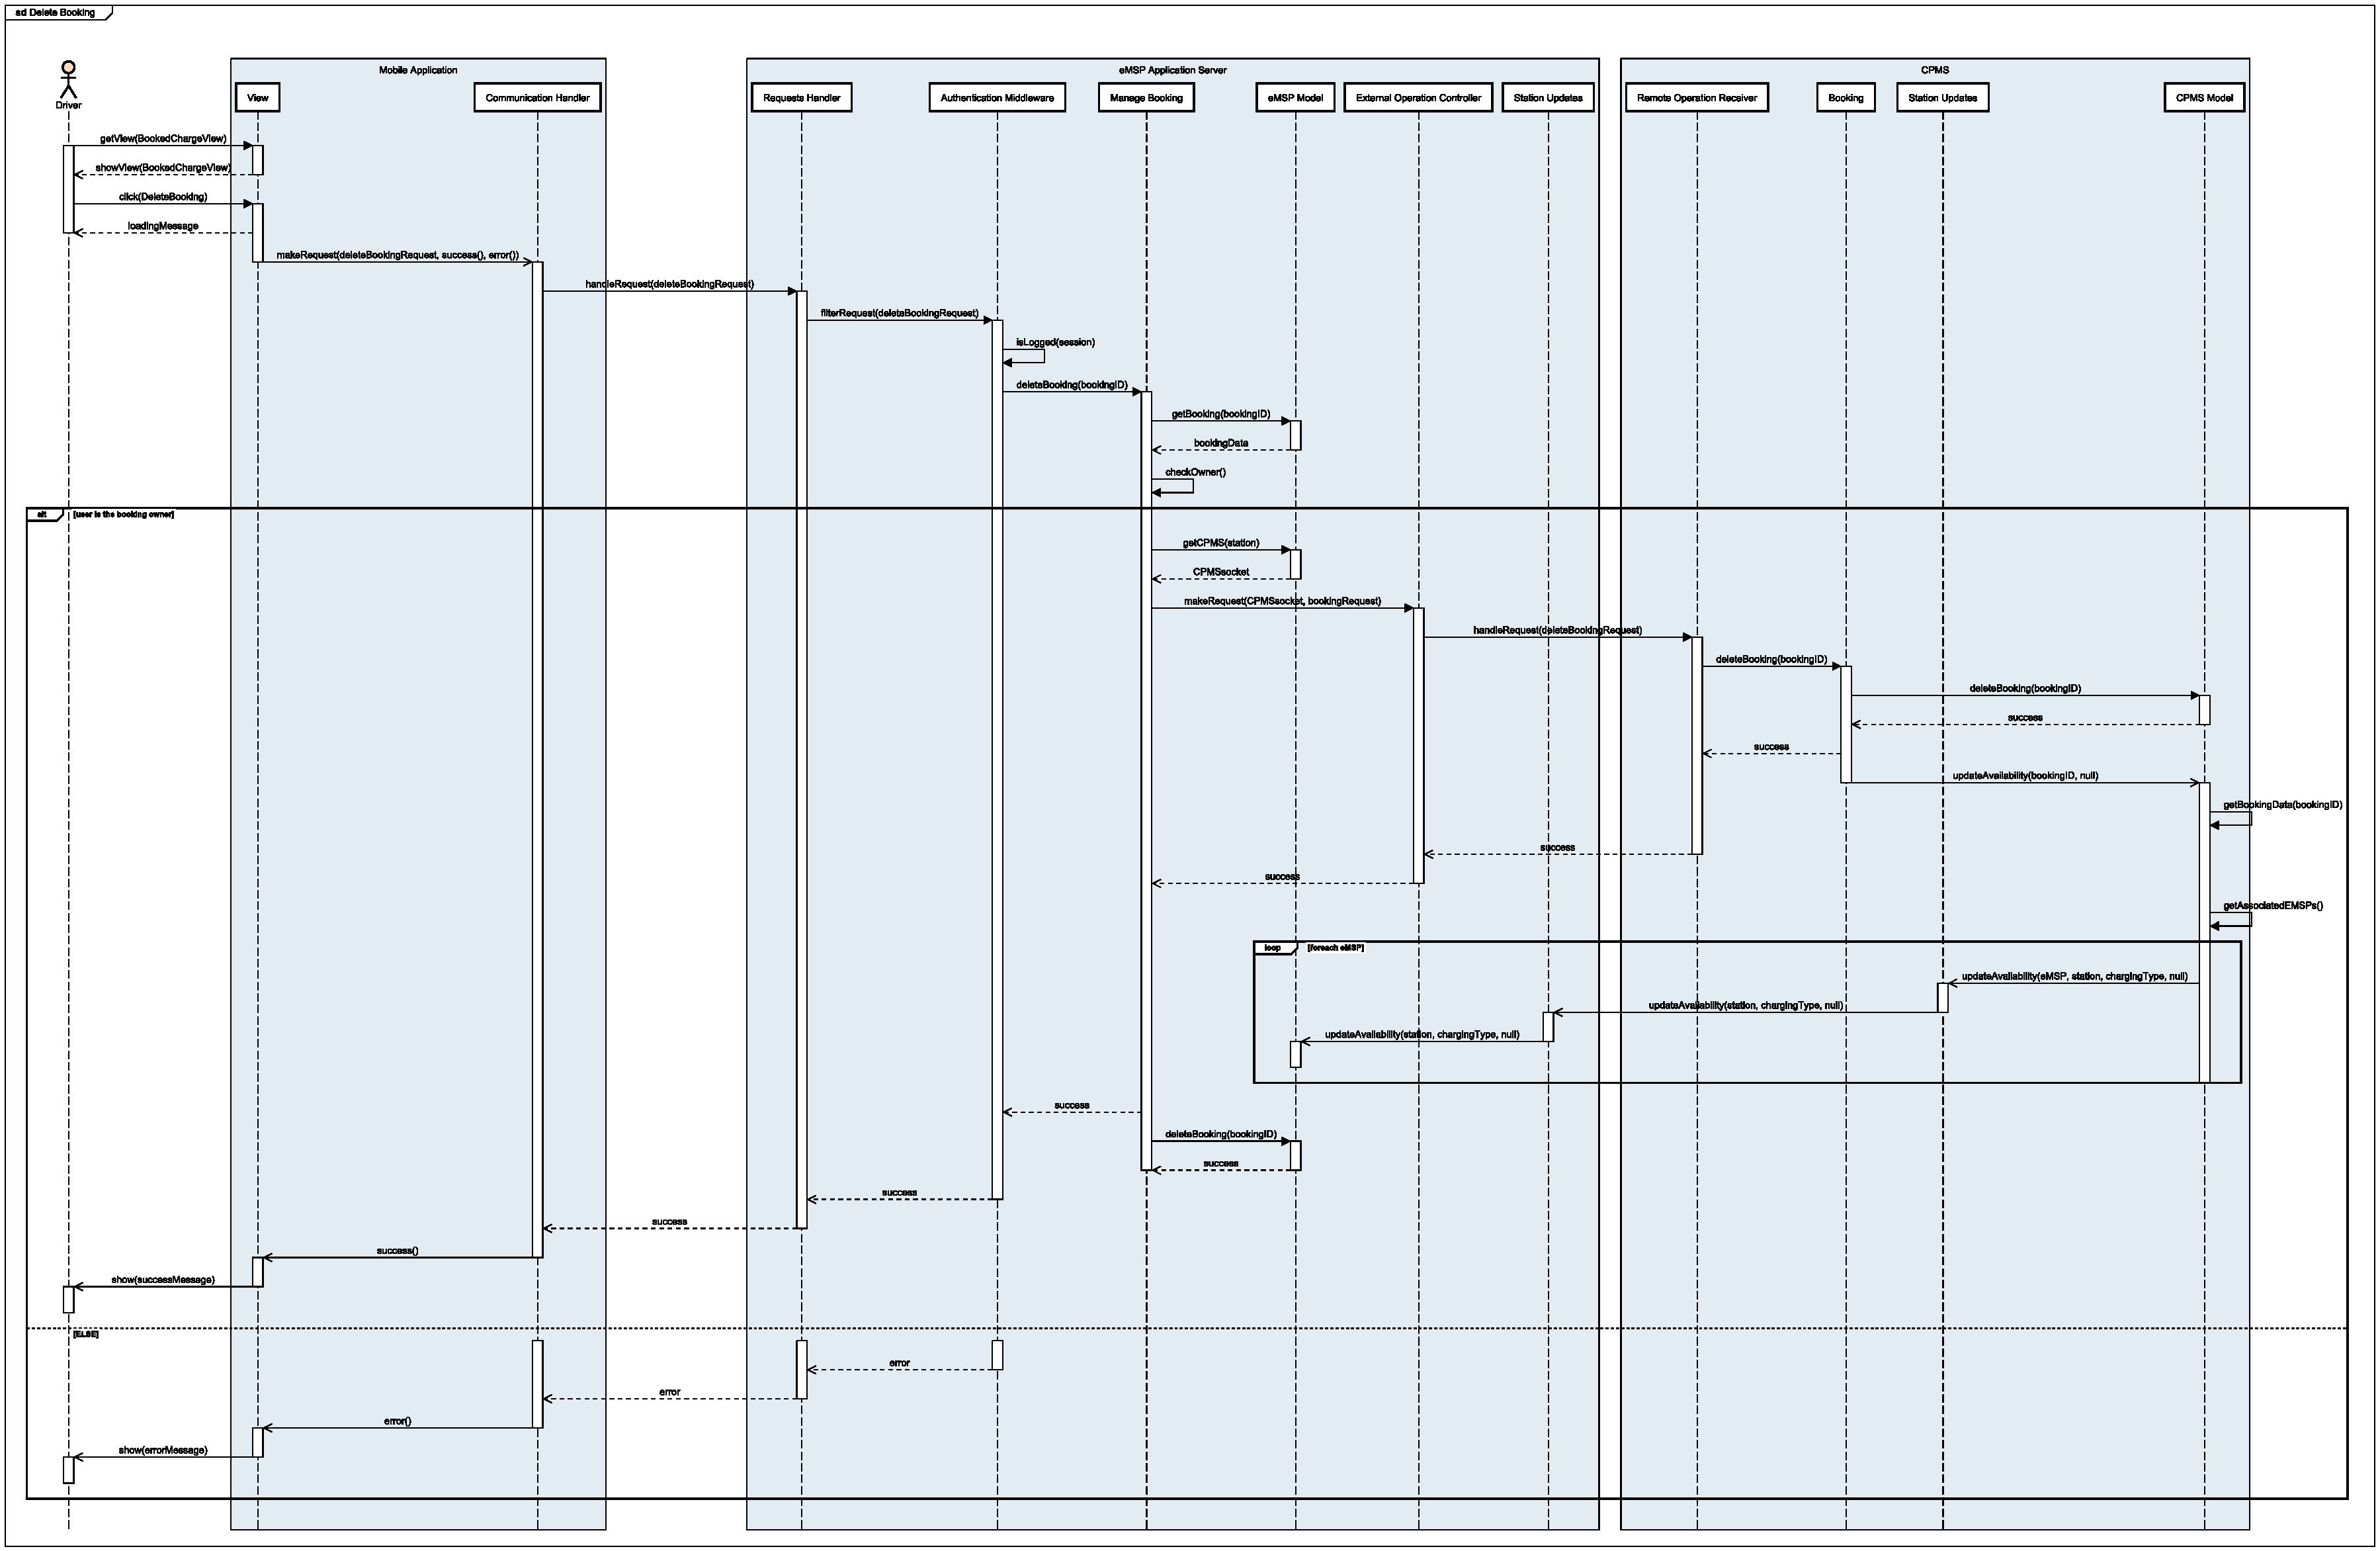
\includegraphics[
                width=\textwidth,
                height=\textheight,
                keepaspectratio]{SeqDia/Delete_Booking}
            \caption{Driver deletes a booking}
            \label{fig:DeleteBooking}
            \end{center}
        \end{figure}
        The figure shows the process of the deletion of a previously created booking. The process is similar to the previous one. When the CPMS updates the availability of a charging station, it sends a null value for the estimated time to indicate that the station is currently available.
        \newpage
        \item \textbf{Suggestion Generation and Notification}
        \begin{figure}[H]
            \begin{center}
            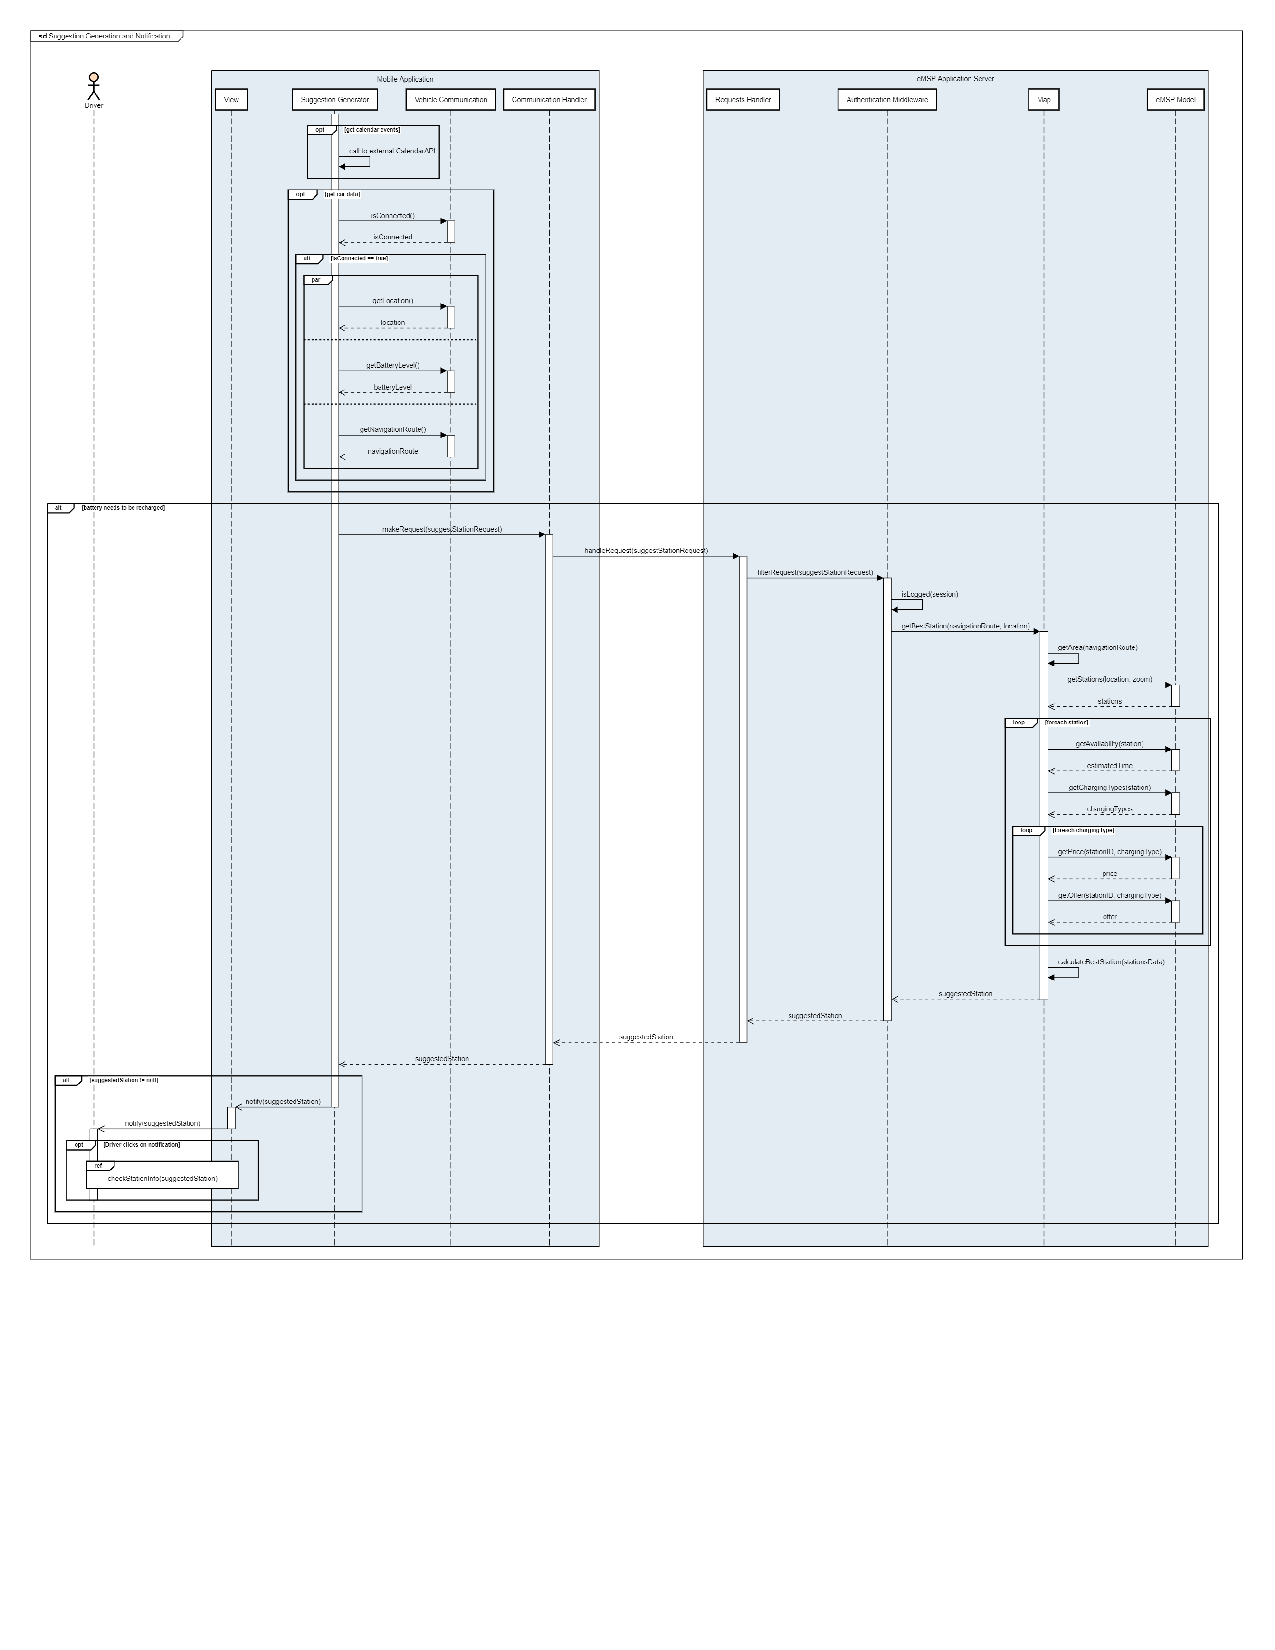
\includegraphics[
                width=\textwidth,
                height=\textheight,
                keepaspectratio]{SeqDia/Suggestion_Generation_and_Notification}
            \caption{Driver receives and opens a suggestion}
            \label{fig:Suggestion}
            \end{center}
        \end{figure}
       The figure shows the process for generating a suggestion. It will be generated on the mobile application by fetching data from the Driver's vehicle, Driver's calendar APIs and eMSP application server (in order to retrieve charging station info). 
       \newpage
        \item \textbf{Start Charging Process}
        \begin{figure}[H]
            \begin{center}
            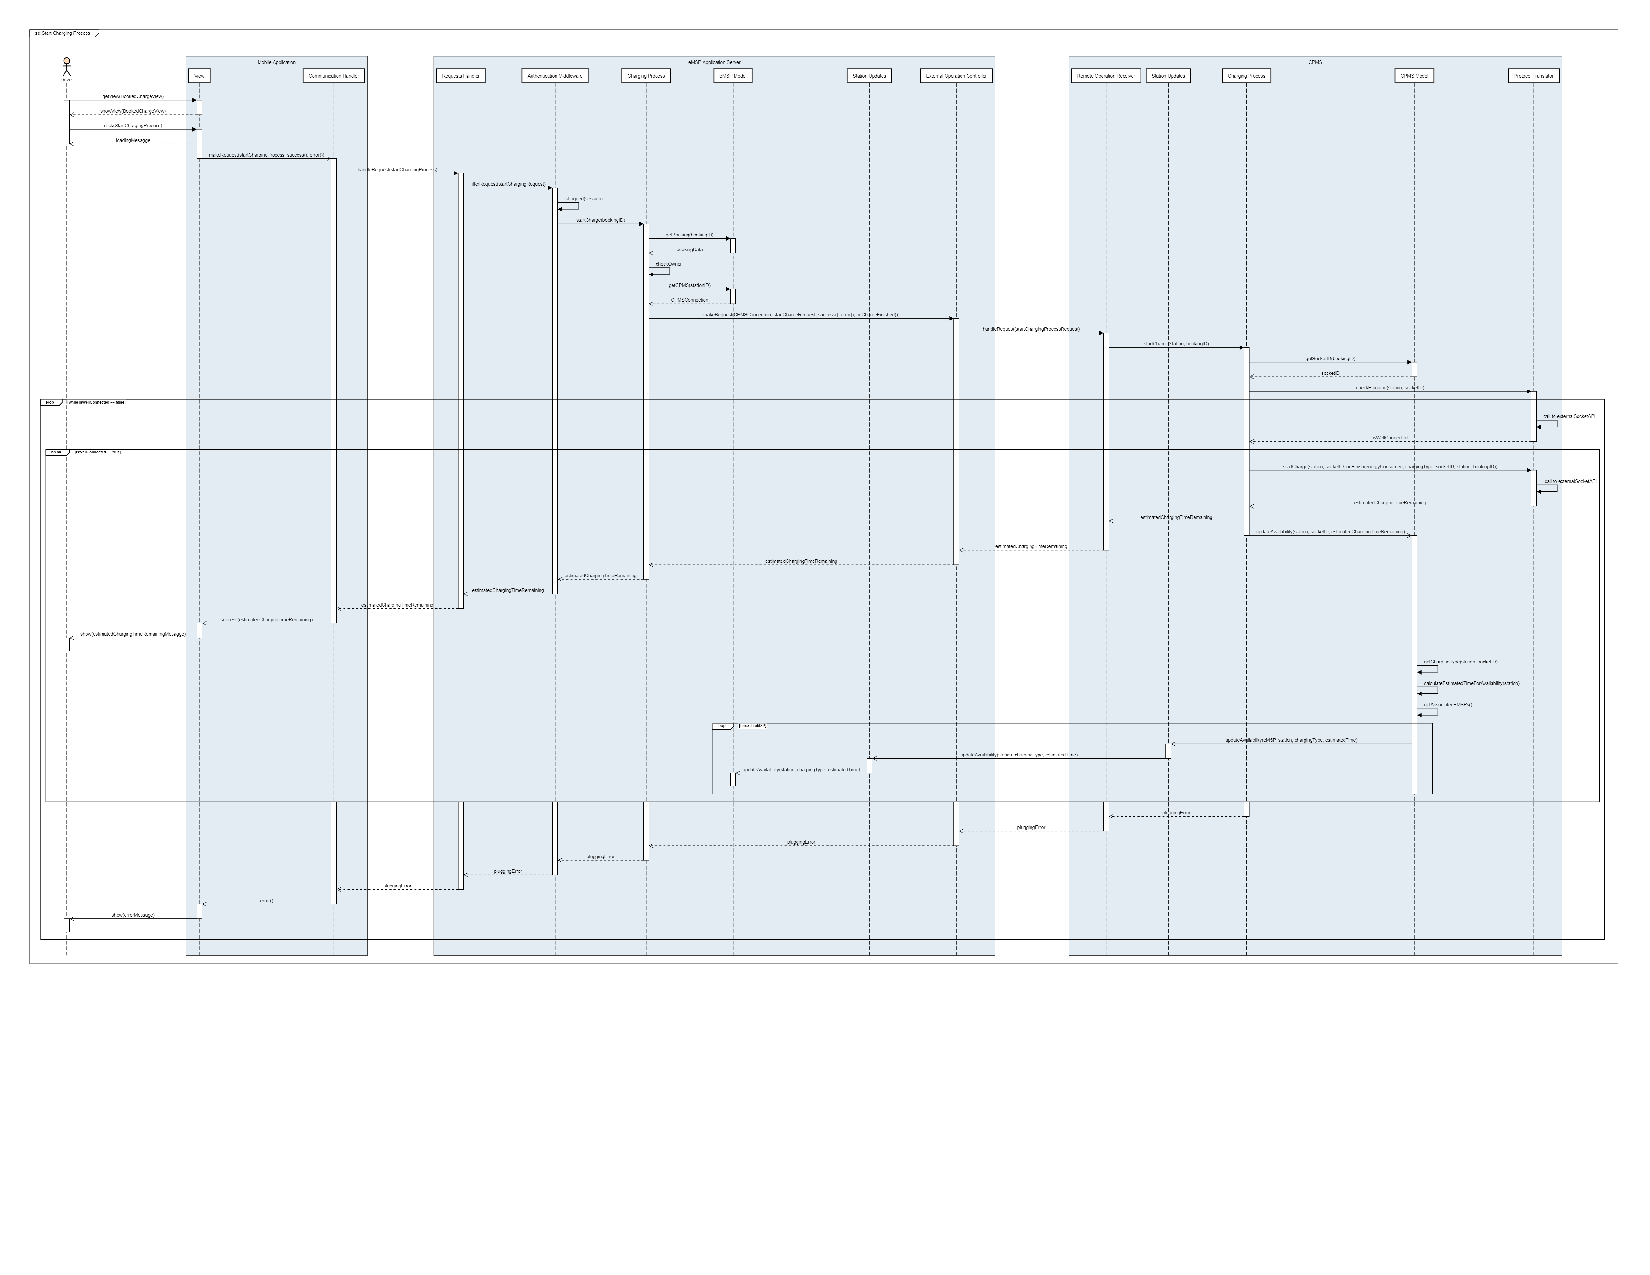
\includegraphics[
                width=\textwidth,
                height=\textheight,
                keepaspectratio]{SeqDia/Start_Charging_Process}
            \caption{Driver starts the charging process}
            \label{fig:StartCharge}
            \end{center}
        \end{figure}
        The figure shows the process for starting a charging process. After the Driver clicks the button, the request will be sent to the eMSP application server and from there, to the specific CPMS that will make a check for correct plugging. The charging process won't start until the car is well connected. After it started, CPMS will answer the eMSP with the estimated time remaining, calculate the new station availability info and update every associated eMSPs if there is any updated data. 
        \newpage
        \item \textbf{Stop Charging Process}
        \begin{figure}[H]
            \begin{center}
            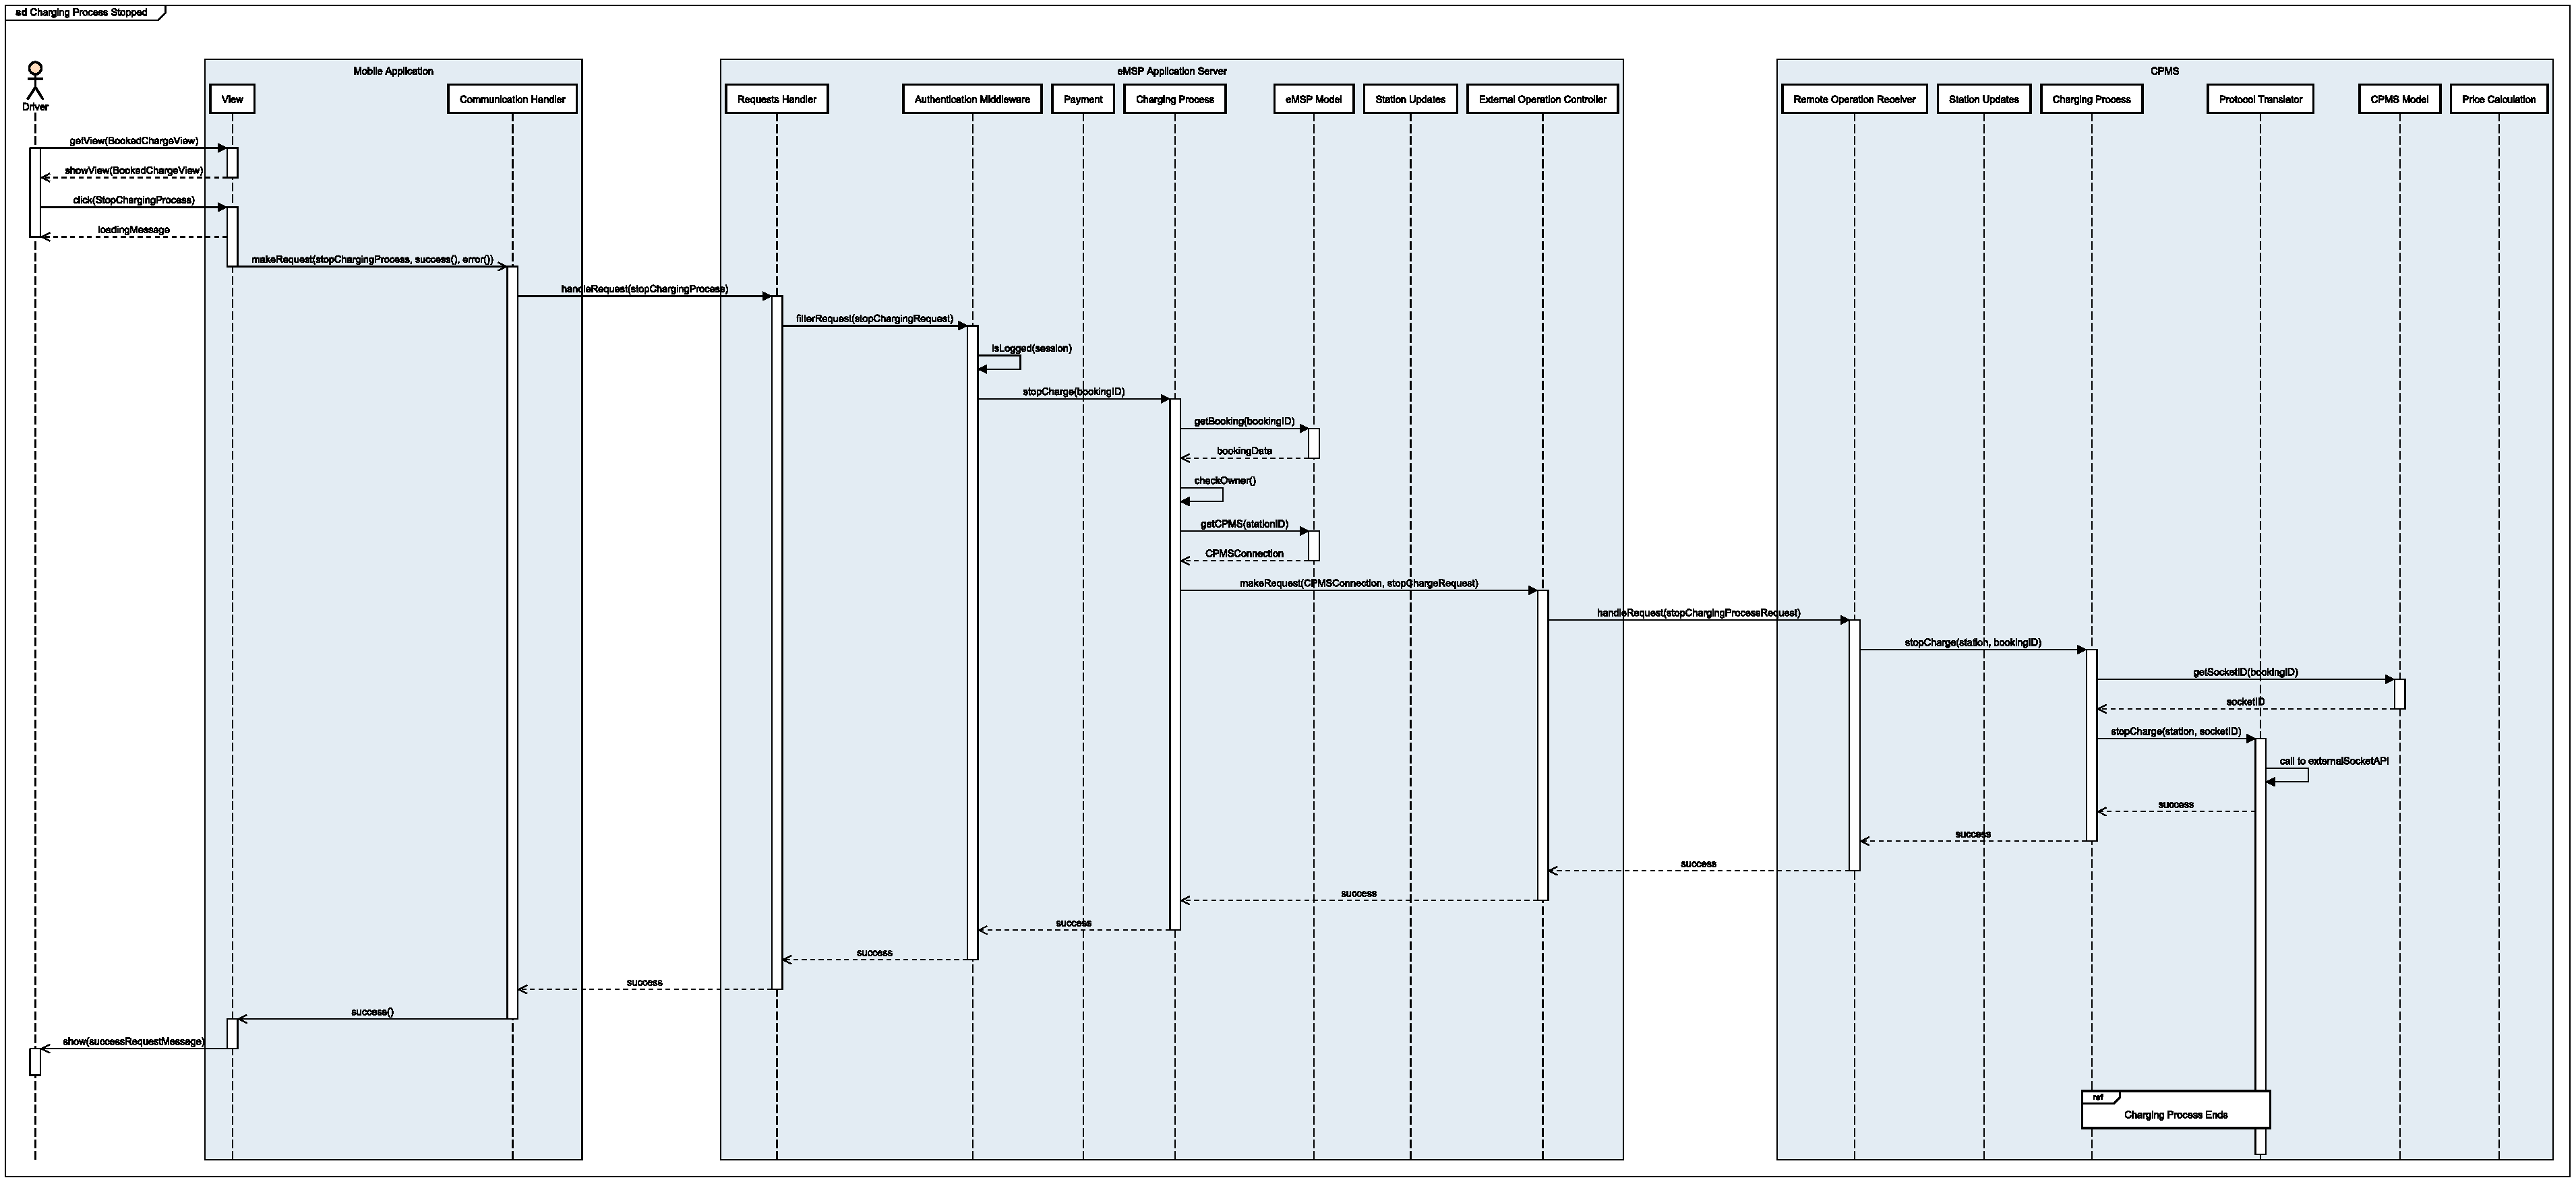
\includegraphics[
                width=\textwidth,
                height=\textheight,
                keepaspectratio]{SeqDia/Charging_Process_Stopped}
            \caption{Driver stops the charging process}
            \label{fig:StopCharge}
            \end{center}
        \end{figure}
        The figure shows the process for stopping a charging process. It starts when the Driver clicks on a specific button. After receiving the response, the user will receive as shown in the following sequence diagram the notification that the charging process has finished.
        \newpage
        \item \textbf{Charging Process Ends}
        \begin{figure}[H]
            \begin{center}
            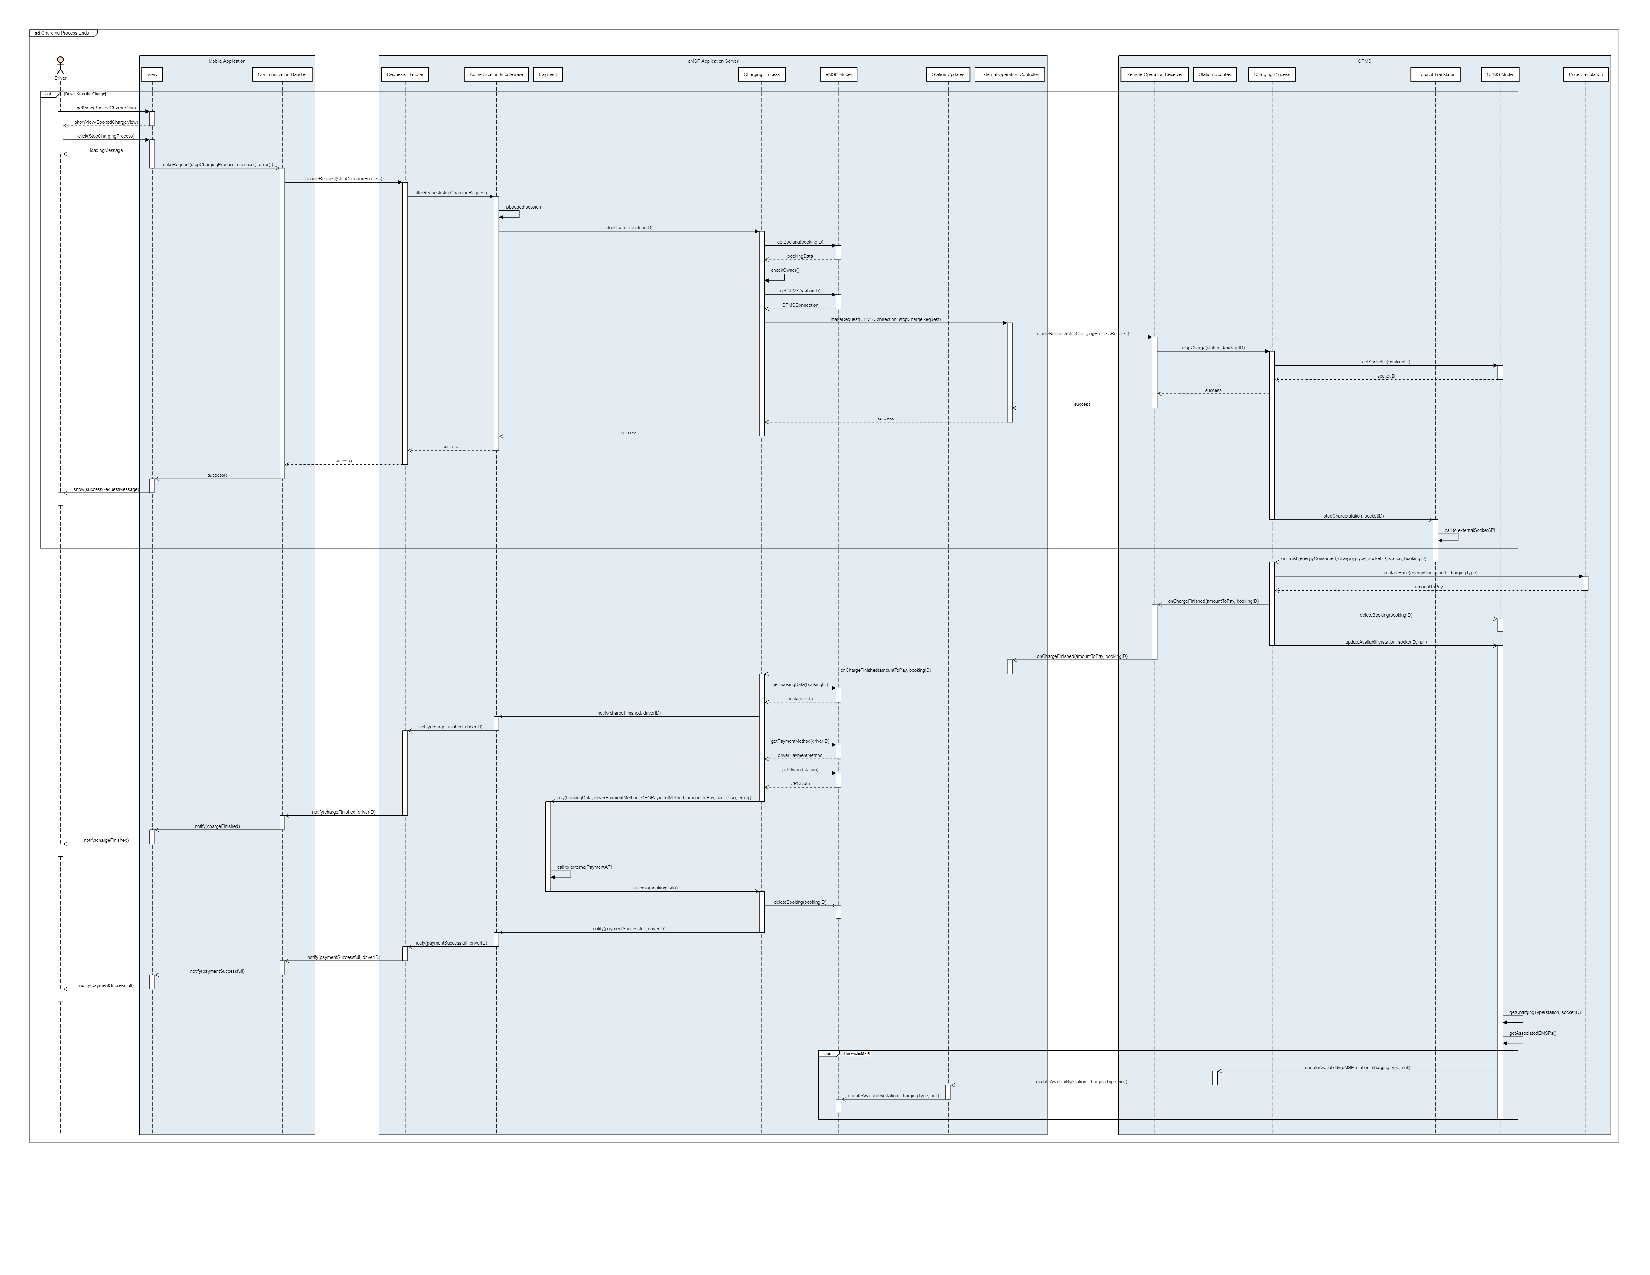
\includegraphics[
                width=\textwidth,
                height=\textheight,
                keepaspectratio]{SeqDia/Charging_Process_Ends}
            \caption{The charging process ends}
            \label{fig:EndCharge}
            \end{center}
        \end{figure}
        The figure shows the process that is executed when a charging process ends. The \textit{Protocol Translator} is going to be the component that will detect the ends of a charging process and will start the corresponding flow. In particular, the CPMS will update every associated eMSPs for charging station availability and then, notify the specific eMSP that made the booking through an async request, with the amount needed to be paid. The eMSP will notify the Driver about the ending of the charging process and once it will finish the payment, it will send another notification to the Driver. This type of async call between eMSPs and CPMSs is advised to be implemented through some sort of callback function such as HTTP webhook. [\ref{webhook}]
        \newpage
        \item \textbf{CPO Authentication}
        \begin{figure}[H]
            \begin{center}
            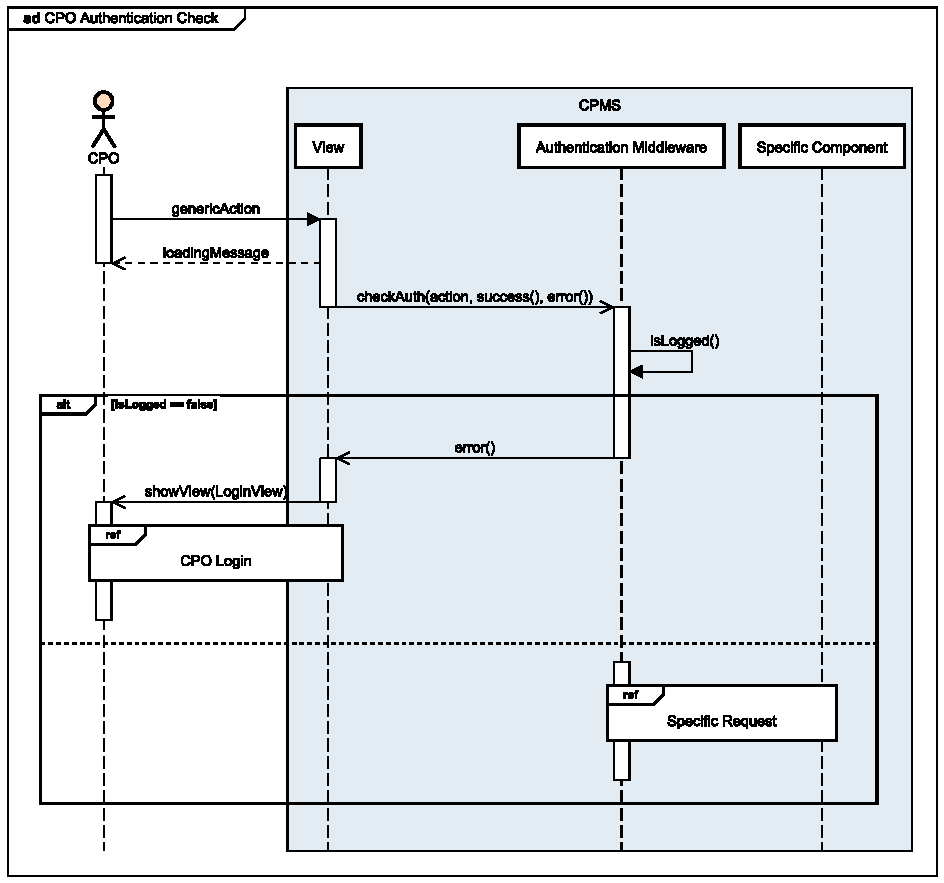
\includegraphics[
                width=\textwidth,
                height=0.45\textheight,
                keepaspectratio]{SeqDia/CPO_Authentication_Check}
            \caption{Authentication of a CPO}
            \label{fig:CPOAuthentication}
            \end{center}
        \end{figure}
        The figure shows the process that is executed for all the requests in order to authenticate CPO. The \textit{isLogged()} function should be internal to the \textit{Authentication Middleware} in order to avoid making calls to the DBSM or to the external eMall API. When the component can no longer check internally the validity, it will redirect the CPO to the Login View. More on this will be explained in the following sequence diagram.
        \newpage
        \item \textbf{CPO Login}
        \begin{figure}[H]
            \begin{center}
            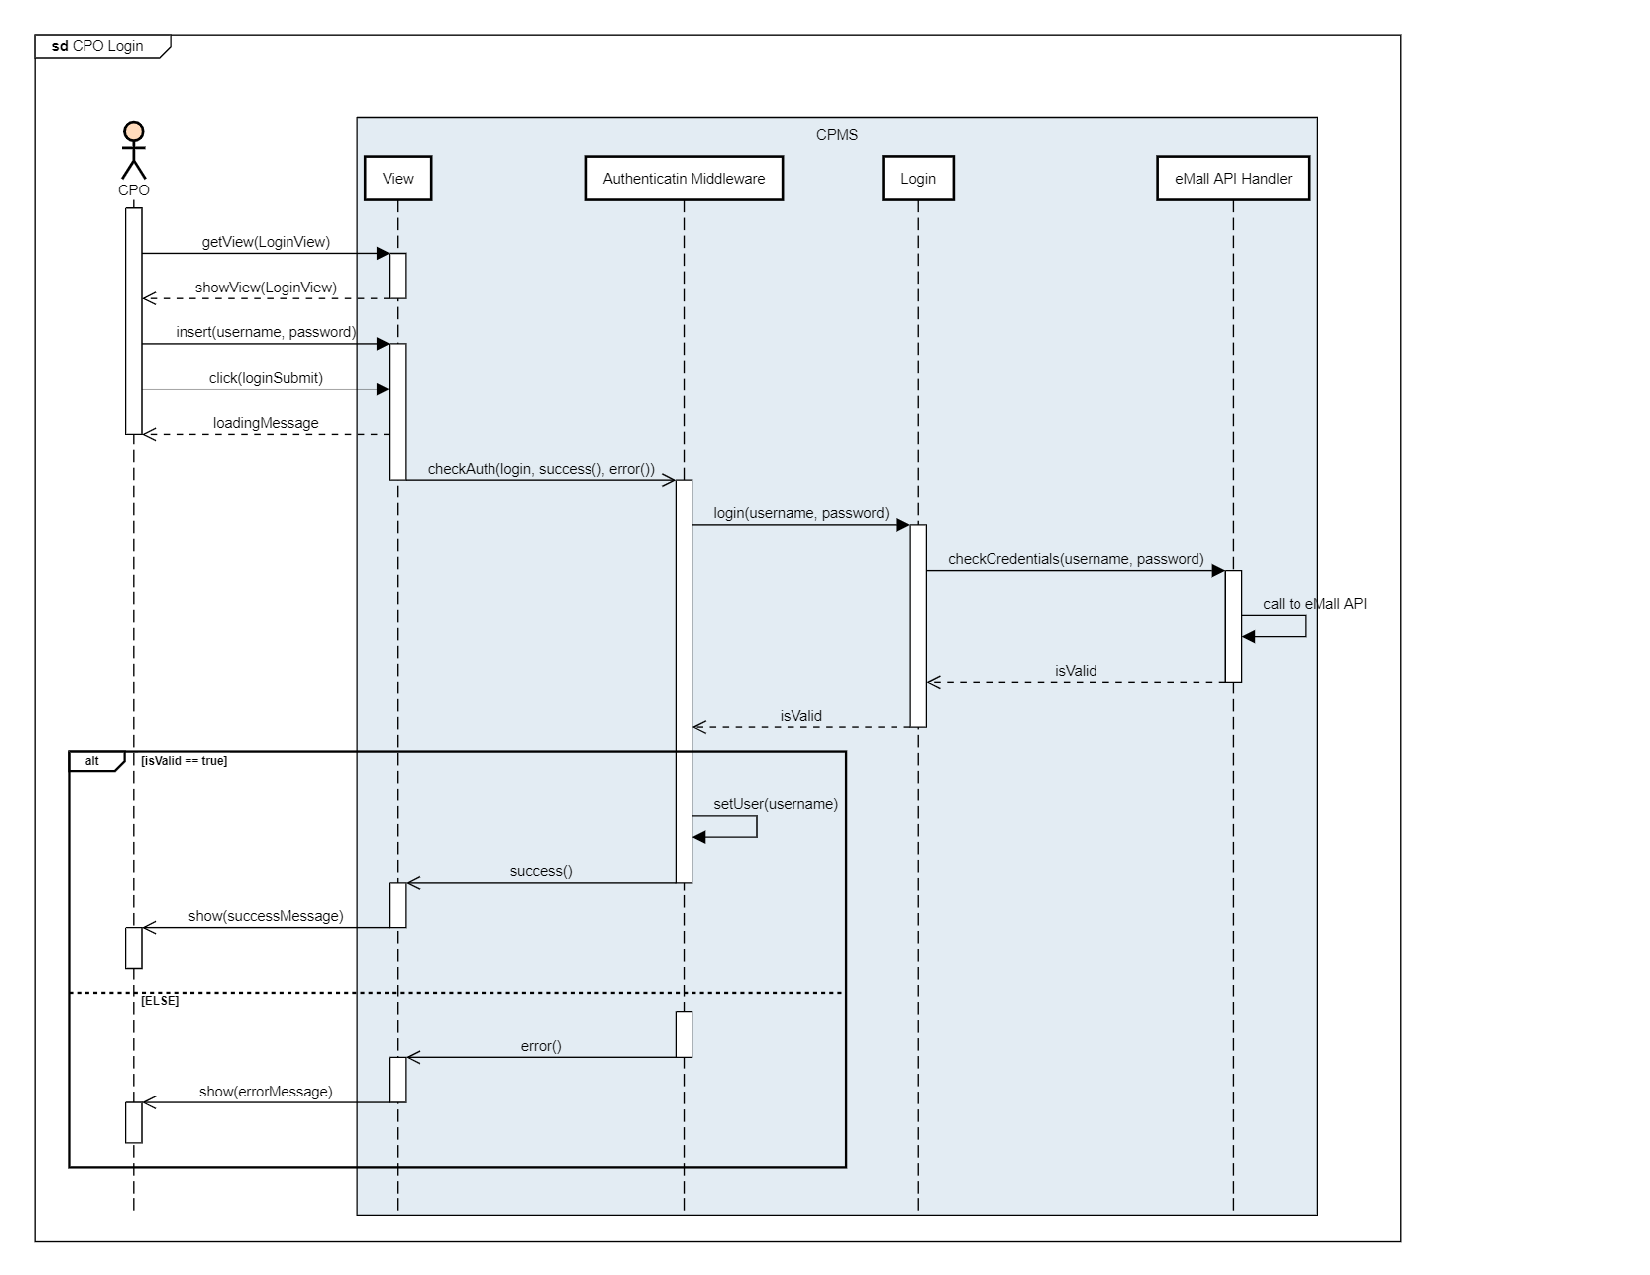
\includegraphics[
                width=\textwidth,
                height=0.45\textheight,
                keepaspectratio]{SeqDia/CPO_Login}
            \caption{Login of a CPO}
            \label{fig:CPOLogin}
            \end{center}
        \end{figure}
        The figure shows the process for authenticating the CPO. Since the credentials are stored on the eMall platform, the CPMS should contact its API in order to perform validation. Once the validation is done, the \textit{Authentication Middleware} should store internally that the CPO is authenticated and use that information when checking the authentication. 
        \newpage
        \item \textbf{View Managed Station Status}
        \begin{figure}[H]
            \begin{center}
            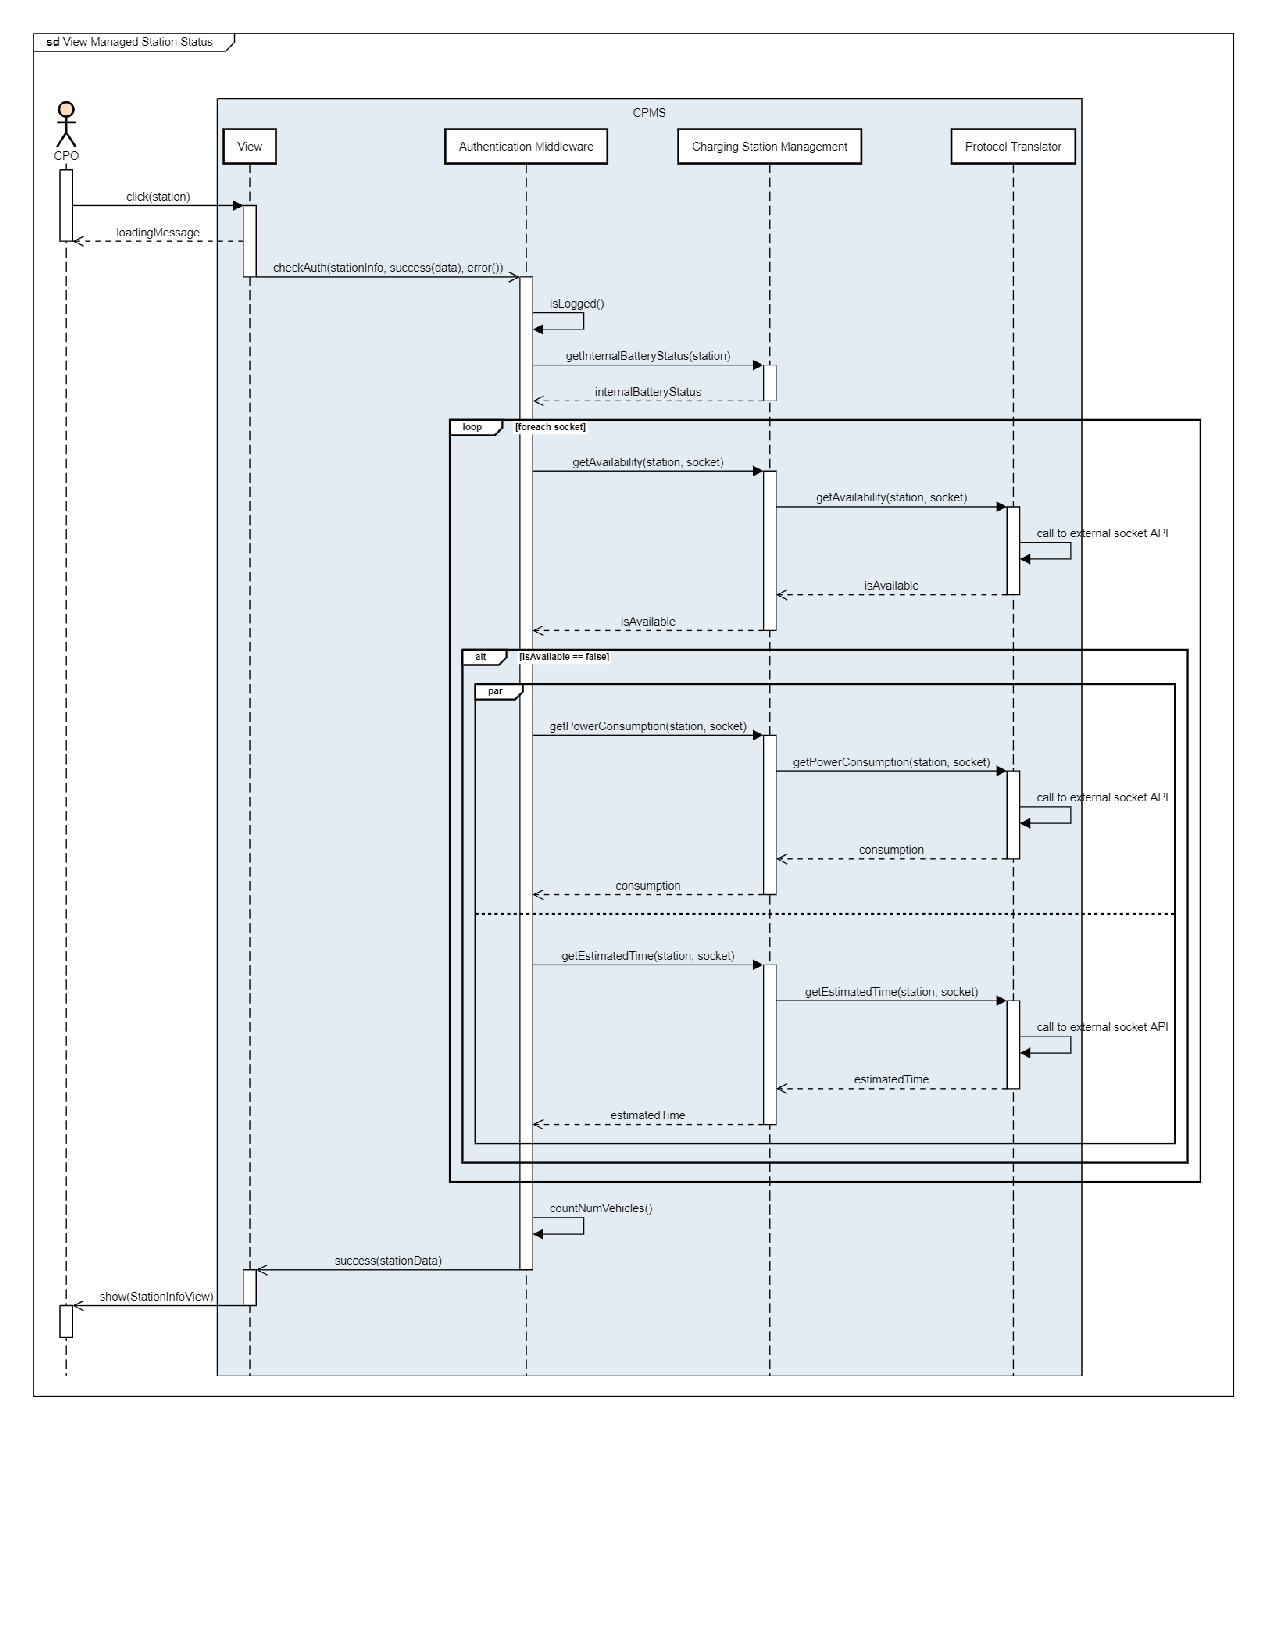
\includegraphics[
                width=\textwidth,
                height=\textheight,
                keepaspectratio]{SeqDia/View_Managed_Station_Status}
            \caption{CPO views a managed station}
            \label{fig:ManageStation}
            \end{center}
        \end{figure}
        The figure shows the process executed when the CPO wants to see the info of one of his stations such as availability, battery status, power consumption, vehicle numbers and estimated time.
        \newpage
        \item \textbf{Add Station To CPMS}
        \begin{figure}[H]
            \begin{center}
            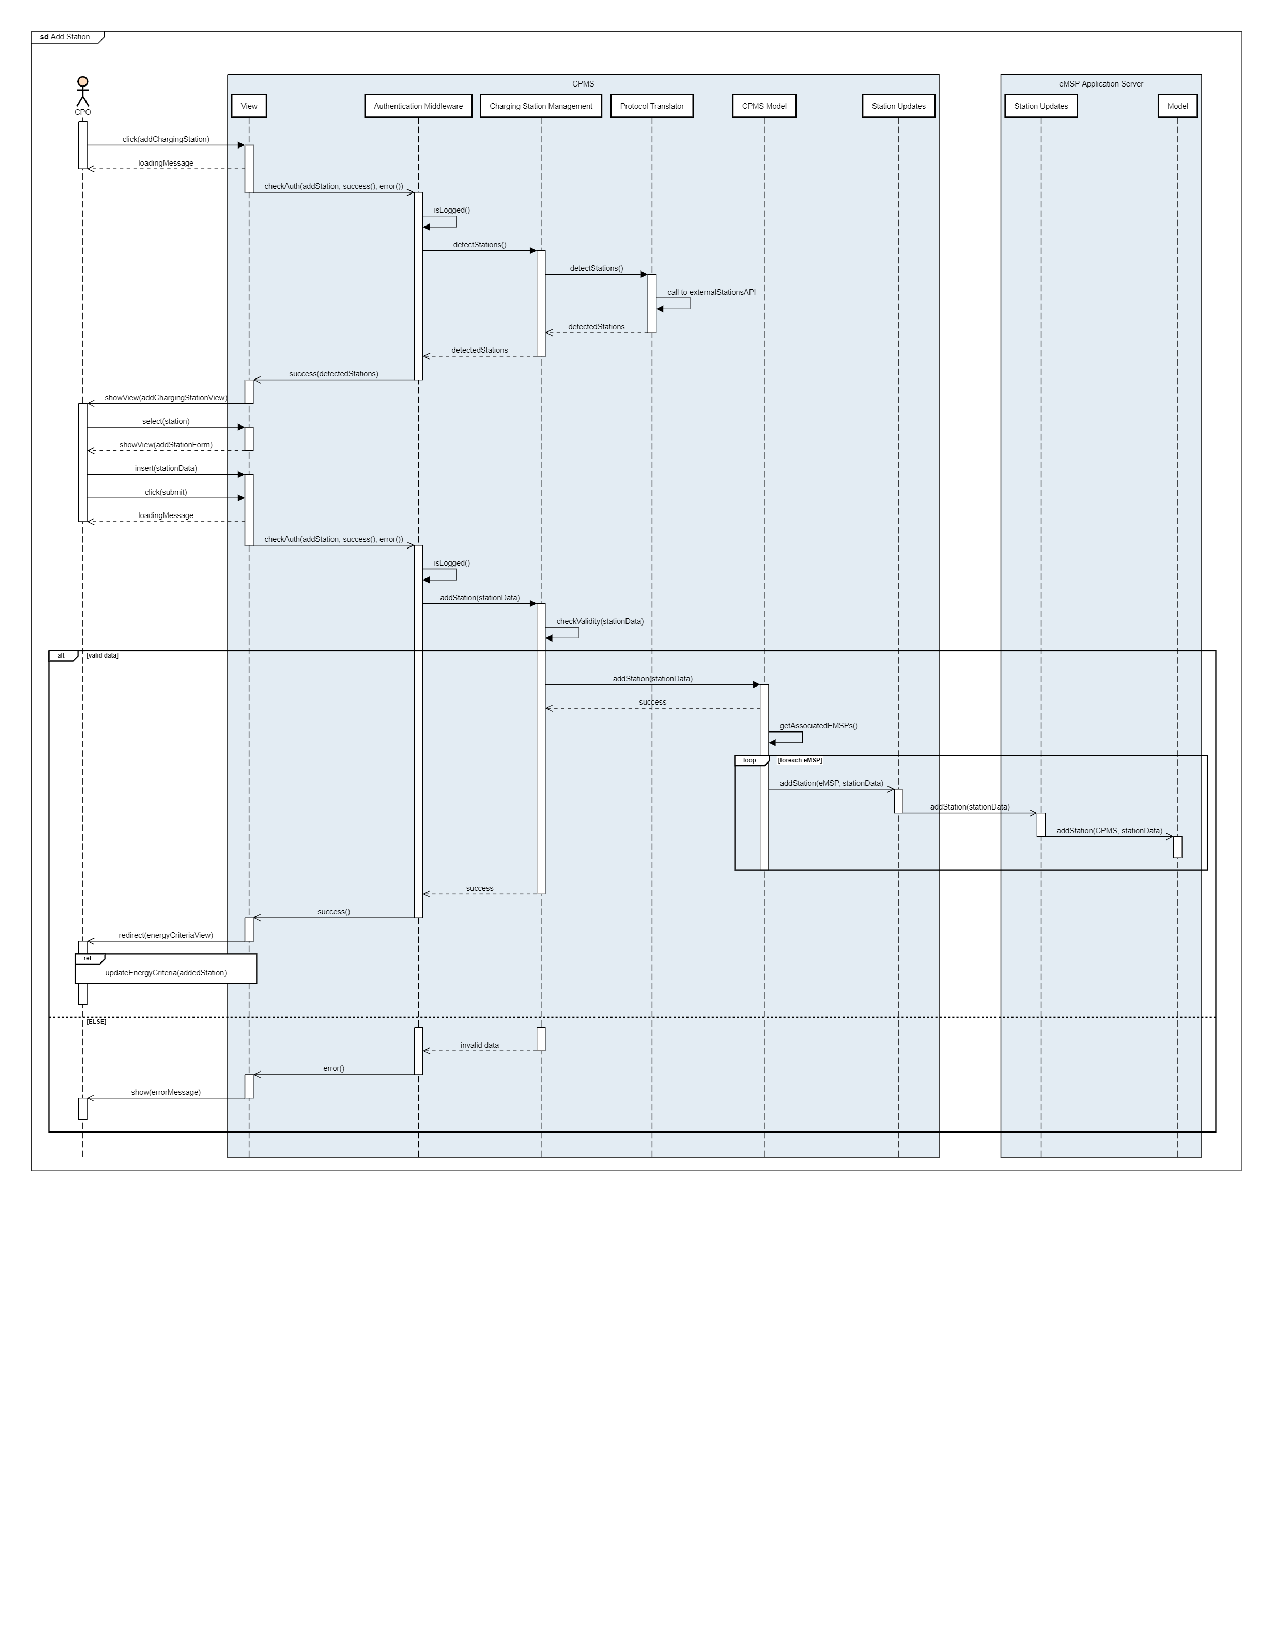
\includegraphics[
                width=\textwidth,
                height=\textheight,
                keepaspectratio]{SeqDia/Add_Station}
            \caption{CPO adds a station}
            \label{fig:AddStation}
            \end{center}
        \end{figure}
        The figure shows the process for adding a new charging station. The CPMS with \textit{Protocol Translator} component will detect the charging station and the CPMS can add one of them by inserting all the required data. Once the station is added, the CPMS will updates all associated eMSPs and then redirect the CPO to the \textit{energyCriteriaView}.
        \newpage
        \item \textbf{Set Offer}
        \begin{figure}[H]
            \begin{center}
            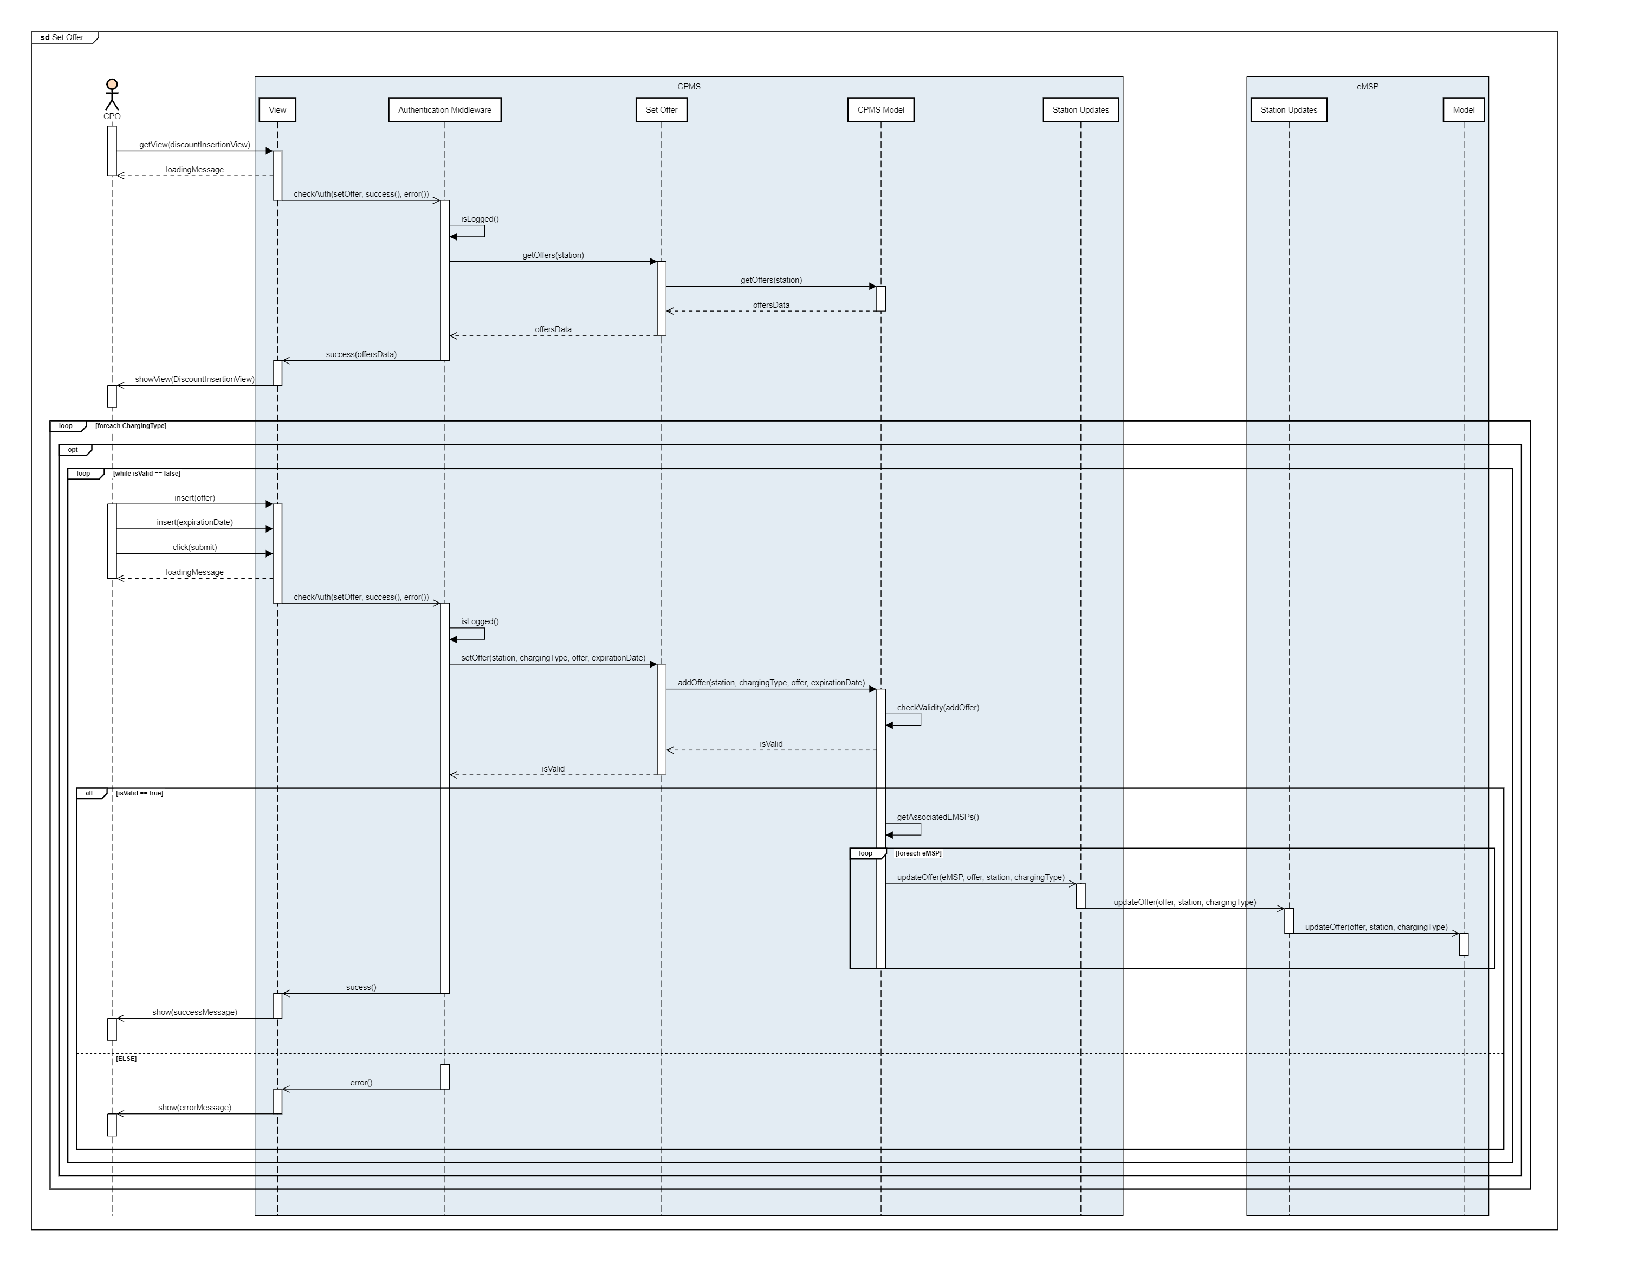
\includegraphics[
                width=\textwidth,
                height=\textheight,
                keepaspectratio]{SeqDia/Set_Offer}
            \caption{CPO sets a new offer}
            \label{fig:SetOffer}
            \end{center}
        \end{figure}
        The figure shows the process when the CPO sets a new offer related to a charging station. After he sets the charging type or discount or expiration date for an offer the CPMS checks the validity and then updates all the associated eMSPs
        \newpage
        \item \textbf{Update Energy Criteria}
        \begin{figure}[H]
            \begin{center}
            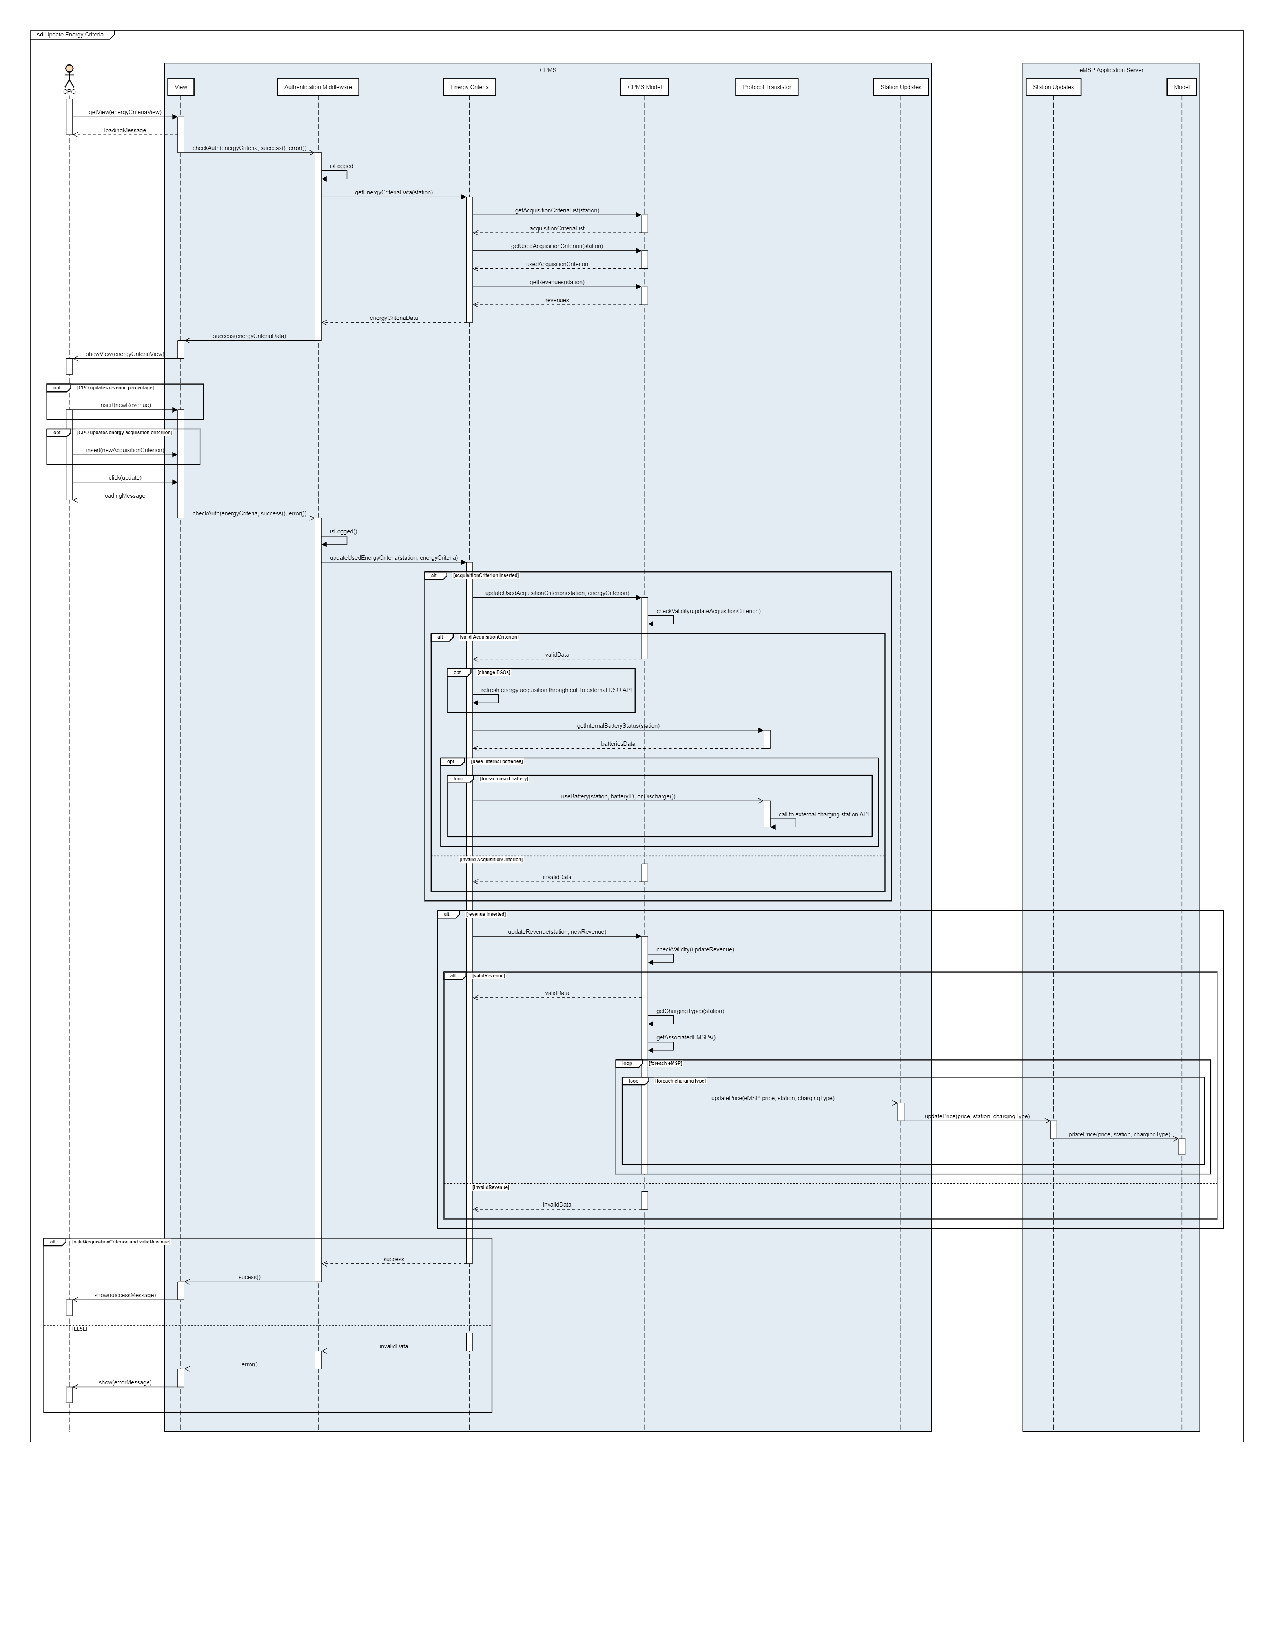
\includegraphics[
                width=\textwidth,
                height=0.85\textheight,
                keepaspectratio]{SeqDia/Update_Energy_Criteria}
            \caption{CPO updates energy criteria}
            \label{fig:UpdateCriteria}
            \end{center}
        \end{figure}
        The figure shows the process when the CPO update the energy criteria: both the acquisition and the revenue. With the acquisition criterion, the CPO can select how the CPMS will automatically take energy from the best energy provider respecting the chosen criterion, meanwhile with the revenue, the CPO can set the percentage of gain that he will get based on the energy price.
        \newpage
        \item \textbf{eMSP Association}
        %\begin{tabbing}
         %   \textbf{Note}: \= In \textit{sendCPOData} is also passed a payment method where the associated eMSP\\
          %  \> will send future drivers' payments.
        %\end{tabbing}
        \begin{figure}[H]
            \begin{center}
            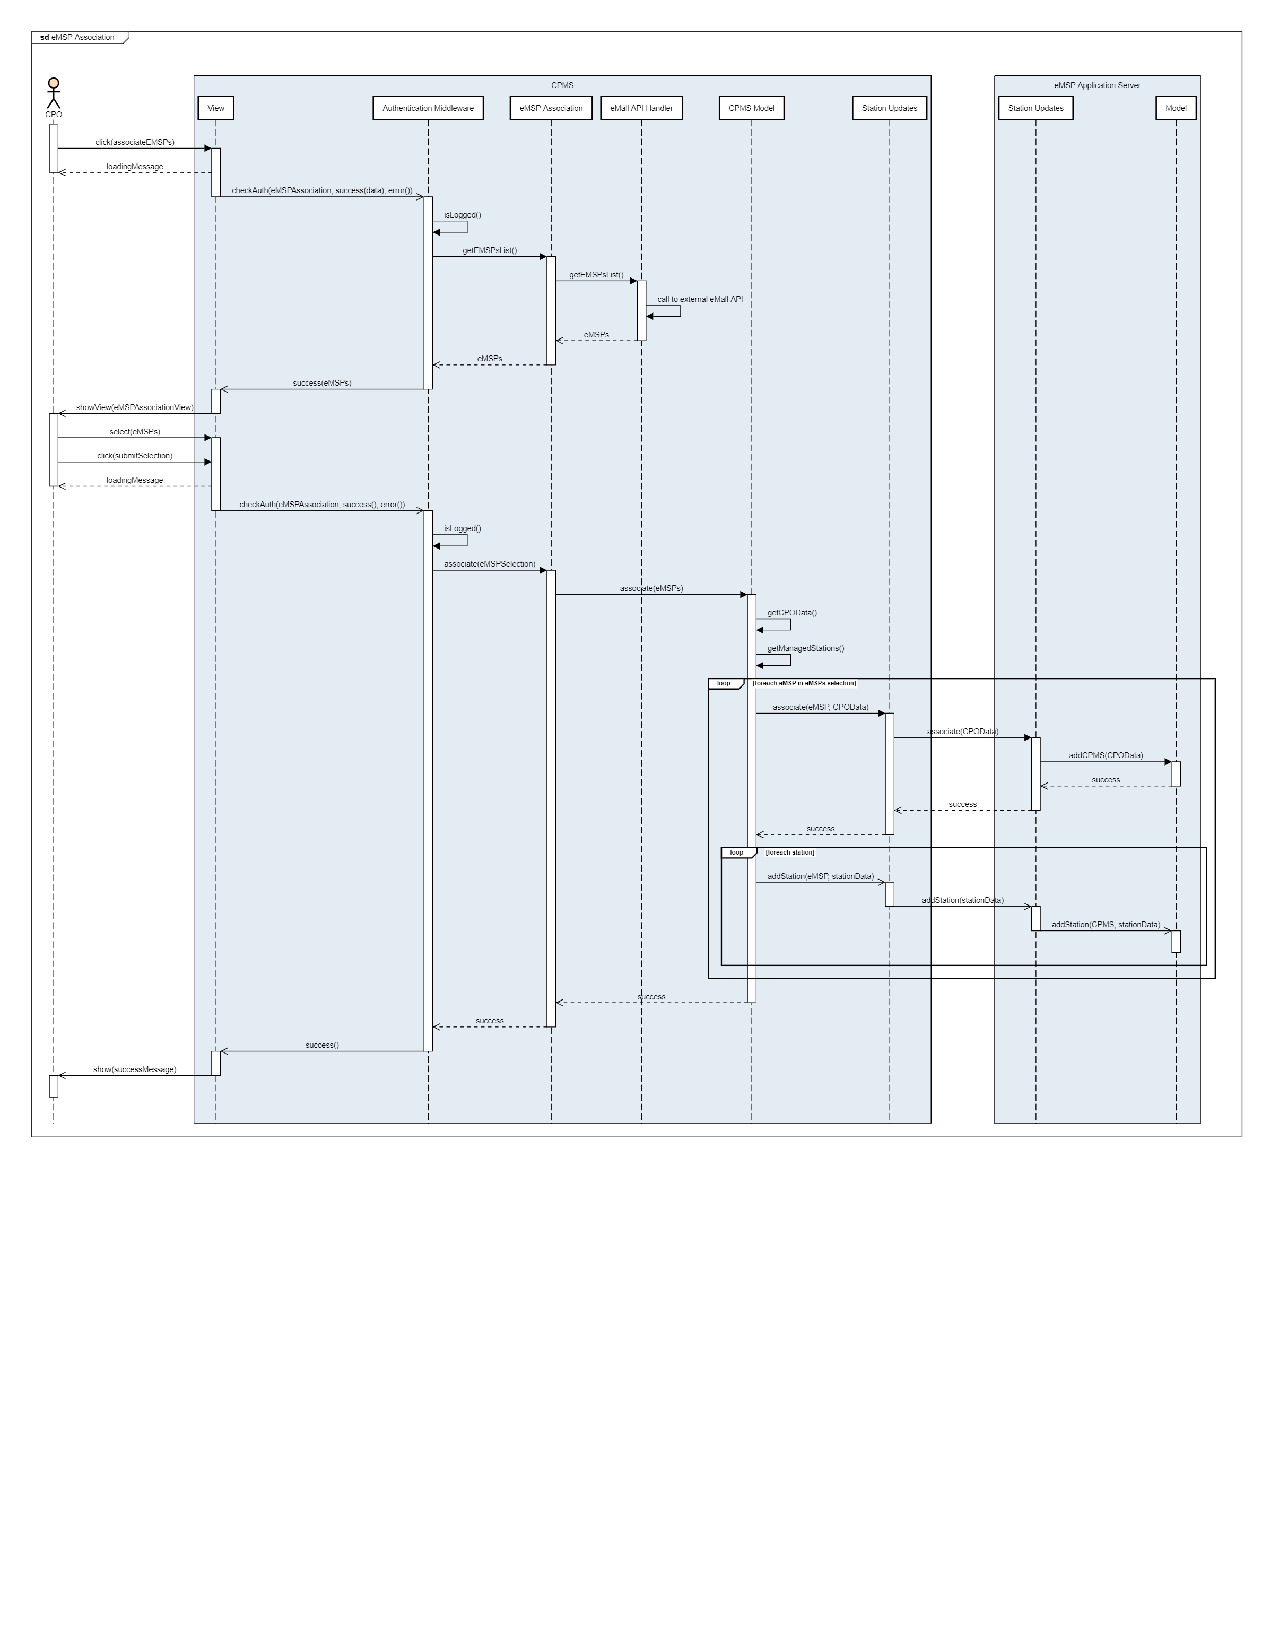
\includegraphics[   
                width=\textwidth,
                height=\textheight,
                keepaspectratio]{SeqDia/eMSP_Association}
            \caption{CPO associates new eMSPs}
            \label{fig:eMSPAssociation}
            \end{center}
        \end{figure}
        The figure shows the process of association between CPMS and eMSP. Without this process, the two subsystems won't be able to communicate. The first time a CPMS associate itself with the eMSP, it will also send all the existing data about its charging station.
\end{enumerate}
\section{Component Interfaces} %AP
\label{sec:componentInterfaces}
\begin{figure}[H]
            \begin{center}
            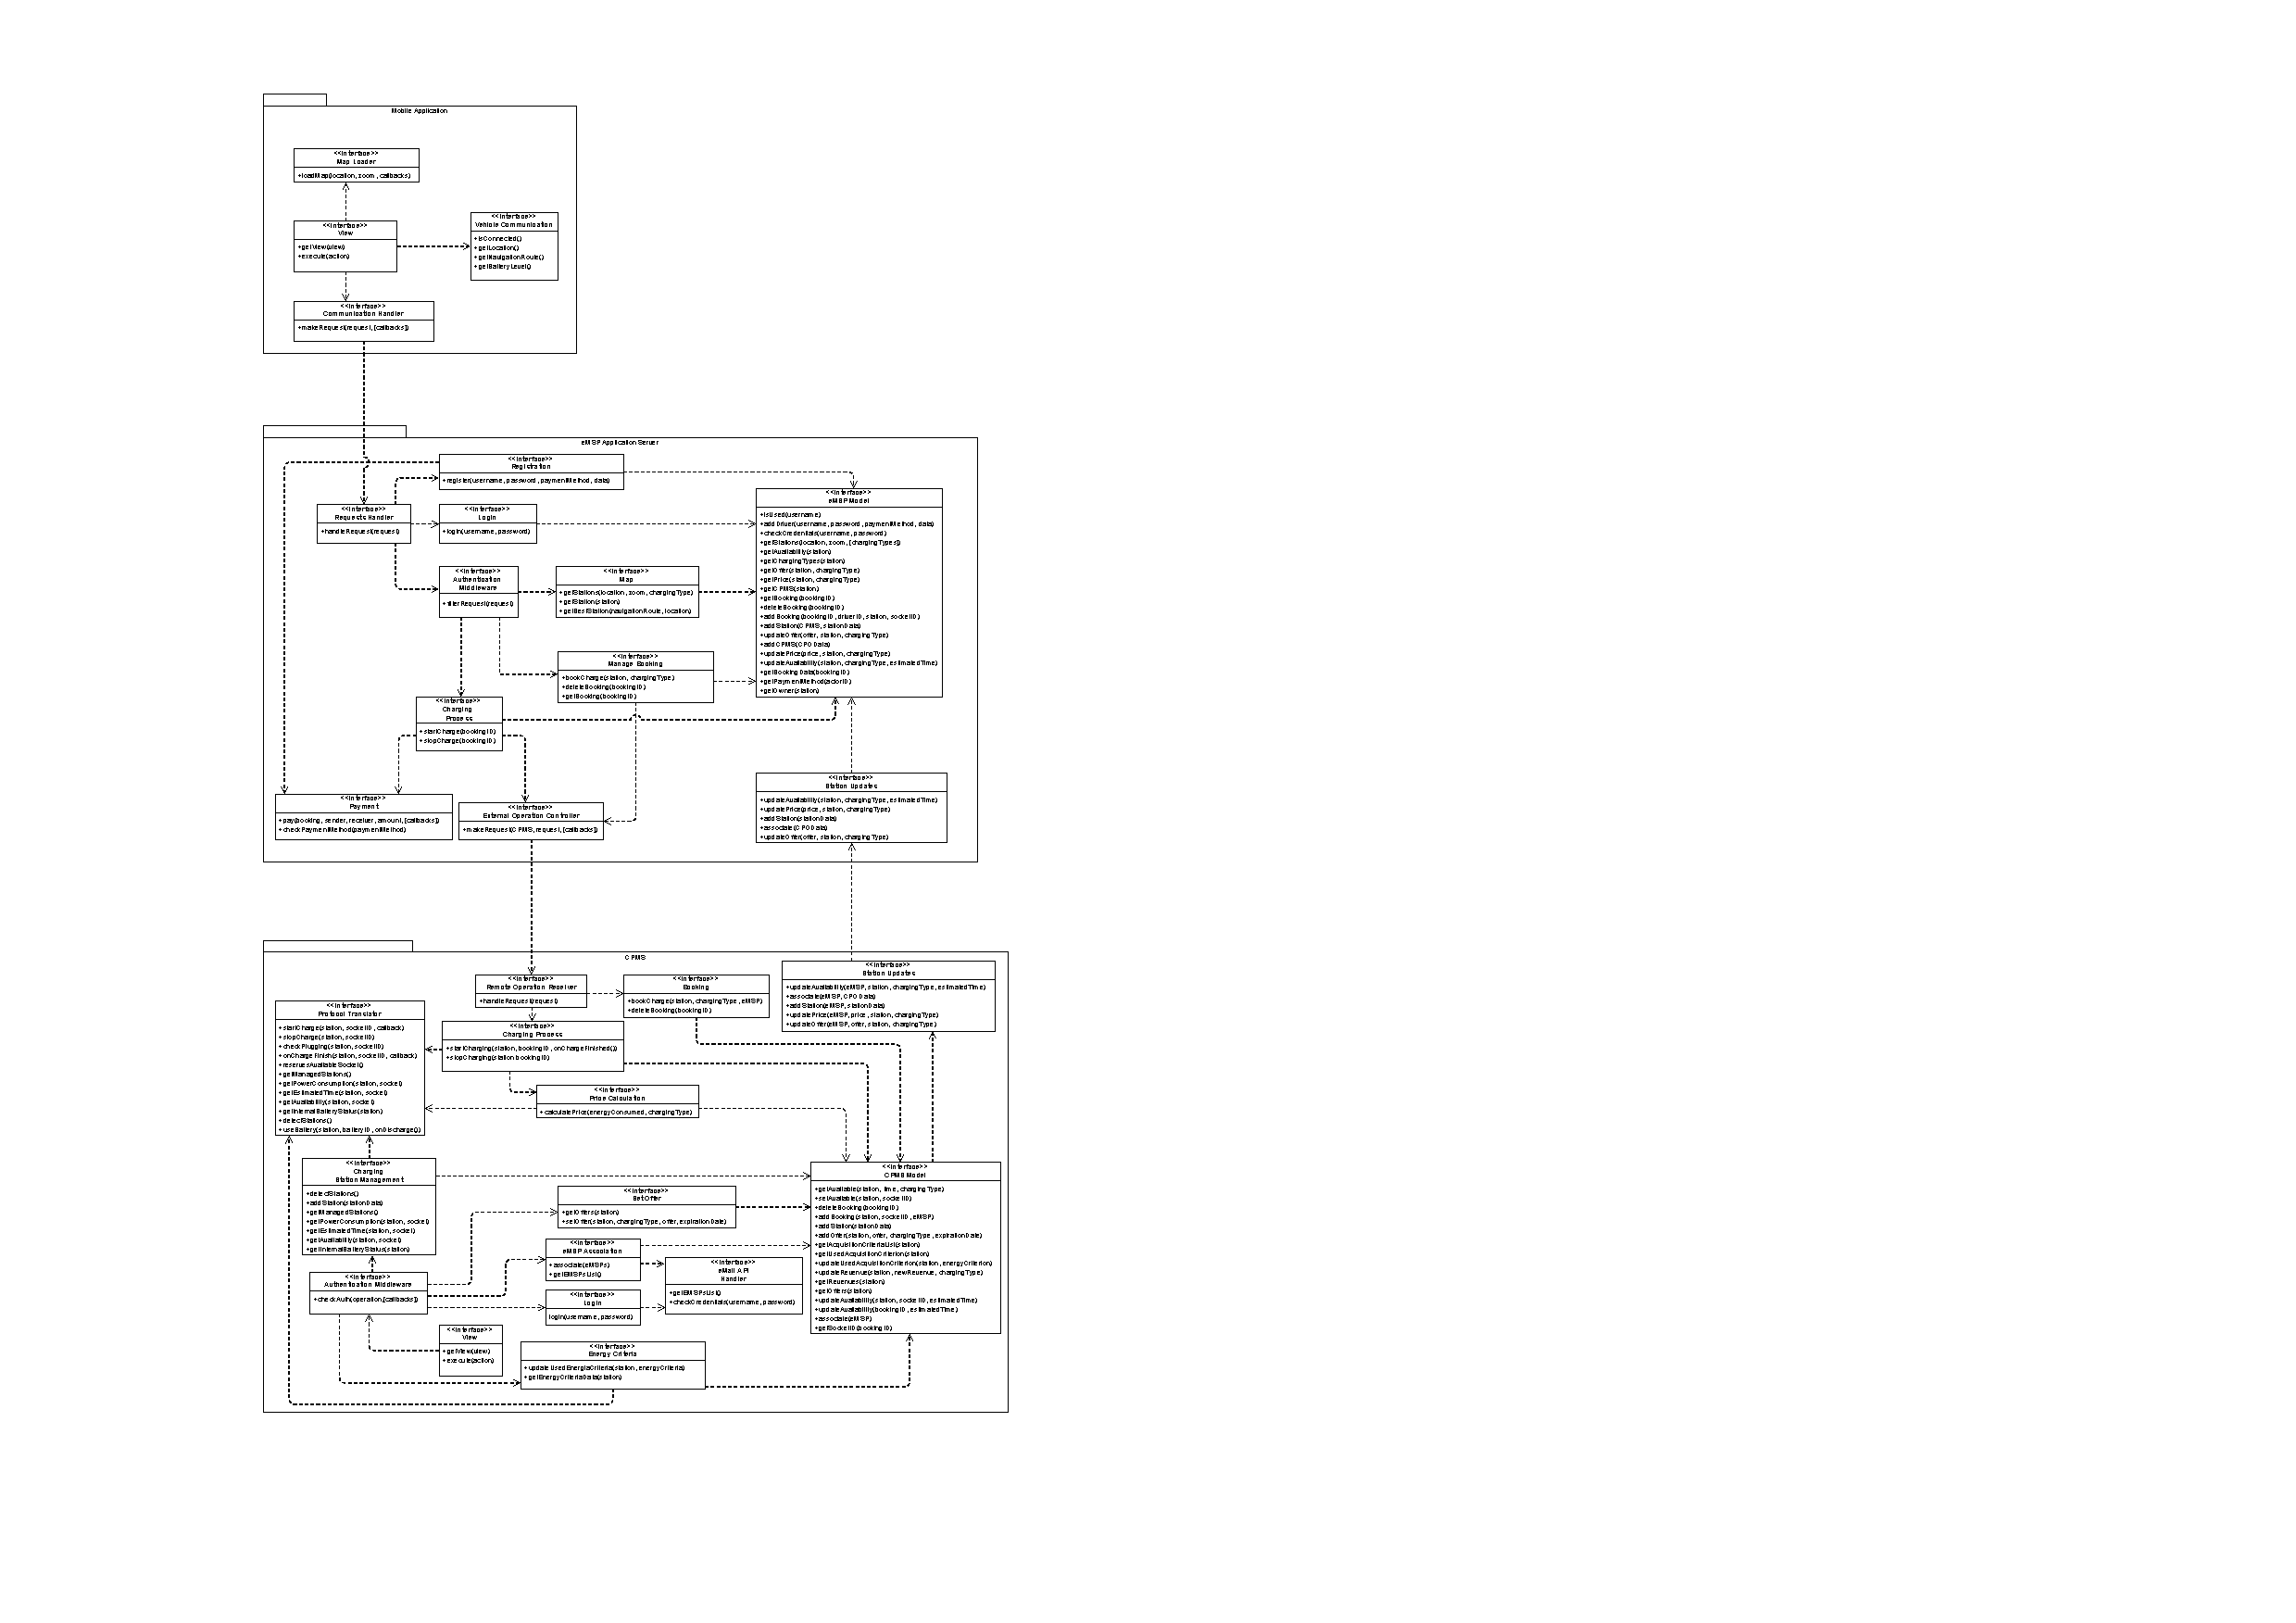
\includegraphics[   
                width=\textwidth,
                height=0.9\textheight,
                keepaspectratio]{Component Interfaces}
            \caption{Component Interfaces Diagram}
            \label{fig:ComponentInterfaces}
            \end{center}
        \end{figure}
\section{Selected Architectural Styles and Patterns} %AS
\label{sec:artchitecturalStylesPatterns}
\subsection{Architectural Styles}
In the overview section, a description is provided of how a three-tier client-server architecture has been used to design the eMSP system, while a monolithic architecture has been used to design the CPMS. For communication between the mobile application, eMSP server, and CPMS, a REST architecture was chosen. In particular, the communication can be integrated using a webhook [\ref{webhook}] to allow for HTTP callbacks.
\label{subsec:architecturalStyles}
\subsection{Patterns}
Recommended pattern to implement the application:
\begin{itemize}

\item \textbf{Model-View-Controller Pattern (MVC) : }It is an architectural pattern which divides
the application into three interconnected parts. It is used to separate how the information is represented inside the system from what the user actually sees. It is a really good and easy pattern to use when a system is based on a three-tier architecture.
\item \textbf{Observer Pattern (OP)}: It simplifies the communications between objects, notifying changes in the state of other specific objects.
\item \textbf {Service-Oriented Architecture (SOA): } This pattern involves building the system as a collection of independent, self-contained services that communicate with each other through APIs. This can make it easier to scale and maintain the system, as changes to one service do not necessarily affect the others
\item \textbf{Model-View-ViewModel (MVVM): } This pattern is similar to MVC, but the ViewModel component is responsible for exposing the data and logic of the model in a way that is consumable by the view. This can make it easier to develop and test the user interface for the mobile application.
\end{itemize}
\label{subsec:patterns}
\section{Other Design Decisions}
This system is designed on the constraint that it will interact with external services. From these external services, the system needs to fetch data or perform operations. In particular, the following are the interfaces that both the eMSP and CPMS are going to use:
\paragraph{Mobile Application}
\begin{itemize}
    \item \textbf{MAP Provider API: } From this interface, the mobile application can fetch the data needed to show the user the location of the station, and the area around it.
    \item \textbf{Calendar API: } From this interface, the mobile application can fetch the data needed to create a more personalized suggestion for the user.
    \item \textbf{Vehicle Connection: } From this interface, the mobile application can fetch the data needed to create a more personalized suggestion for the user.
\end{itemize}
\paragraph{eMSP}
\begin{itemize}
    \item \textbf{Payment API: } From this interface, the eMSP can handle all the payments without needing to implement a new payment system.
    \item \textbf{DBMS API: } From this interface, the eMSP can perform operations in order to store data and read them.
\end{itemize}
\paragraph{CPMS}
\begin{itemize}
    \item \textbf{External Charging Station/Socket API: } From this interface, the CPMS can communicate with charging stations or sockets in order to perform operations or receive notifications about a specific event happening.
    \item \textbf{eMALL API: } From this interface, the CPMS can fetch the data of all the eMSPs in order to associate itself with them and also check the authenticity of a CPO.
    \item \textbf{DSO API: } From this interface, the CPMS can fetch all the information exposed by a DSO about the energy. It is needed to remind that all the DSOs have homogenous APIs
    \item \textbf{DBMS API: } From this interface, the CPMS can perform operations in order to store data and read them.
\end{itemize}
\label{sec:otherDesign}
